\documentclass[12pt]{article}
\usepackage{amsmath}
\usepackage{amsfonts}
\usepackage{bm}
\usepackage[english]{babel} 
\usepackage{xcolor}
\usepackage{textcomp}
\usepackage{graphicx}
\usepackage{natbib} % Powerful citation management
\bibpunct[; ]{(}{)}{,}{a}{}{;} % Custom minimal bibliography styling
\renewcommand{\baselinestretch}{2}\normalsize
\author{Pierre}
\title{Paper NA}
\date{\today}

\begin{document}

\maketitle

\section{Introduction}

\begin{figure}[p]
	\centering
	\centerline{\includegraphics[viewport=180 340 480 570,clip=true,width=\linewidth]{figures/Geologicalmap_Clouzet.pdf}}

	% bb=llx lly urx ury :


	\caption{\baselineskip 18pt
	Large scale Precambrian architecture of North America (modified from \cite{whitmeyer2007tectonic}. Colours indicate ages of different regions, as shown in the legend. The stable cratonic core is defined by the Rocky Mountain Front to the west (dashed dark grey line), defined by the surface trace of deformation), and the appalachian fron to the east (solid light red line). The solid blue line demarcates the westward extent of the Grenville/Llano Front. The solid red line along the Cordillera province demarcates the breakup of Rodinia. Solid green lines indicate tectonic plate boundaries. Abreviations are as follows: RW, re-worked; GBA, Great Bear Arc; BHT, Buffalo Head Terrane; Taltson, Talston Arc; Rimbey, Rimbey Arc; Tornagat, Torngat Arc; L.B.A, Little Belt Arc; LRA; THO, Trans-Hudson Orogen; RGR, Rio Grande Rift; Reelfoot, Reelfoor Rift; Kwn.R, Kewanowan Rift; Sask, Sask Craton; WY, Wyoming Province; Med. Hat., Medicine Hat Block; Grt. Rhy, Granite–Rhyolite Province; Grenville, Grenville Province.
	}

	\label{mapgeol}

\end{figure}

The North American continent consists of an ancient cratonic core, formed during the Archean, that has not been subjected to orogeny for at least 1.8 Ga, bordered to the southeast and east, by progressively younger, stable, Proterozoic provinces \citep{hoffman1988united}. In the west, the Rocky Mountain Front (RMF) separates the Proterozoic and Archean shield from younger, tectonically active provinces (Fig.~\ref{mapgeol}). This relatively regular configuration makes North America an ideal target for seismic tomography, to investigate the relationship of lithospheric and asthenospheric structure to the geological features observed at the surface. 

Differences in the seismic velocity structure between the craton and the western US extending down to at least 200 km were established already in the 1960's and 70's from the first studies of teleseismic P and S wave travel time anomalies  \citep[e.g.][]{cleary1966analysis,herrin1968regional,poupinet1979relation}, the first tomographic images based on P and S travel times \citep{romanowicz1979seismic} and long period surface waveforms \citep{woodhouse1984mapping}, as well as contrasted velocity-depth profiles obtained from the modeling of shear body waveforms at relatively short distances \citep[e.g.][]{grand1984upper}. More recent body wave tomographic models have added considerable details to these images \citep{sigloch2011mantle,burdick2014model,porritt2014seismic,porritt2015lithospheric}

Lateral variations in absolute velocities can be inferred from shear wave tomography, at scales from global \citep[e.g.][]{su1994degree,megnin2000three,shapiro2002monte,panning2006three,kustowski2008anisotropic,ritsema2010s40rts,lekic2011inferring,debayle2012global,schaeffer2013global} to continental \citep{lee2005surface,yuan20113,yuan2014lithospheric,schaeffer2014imaging}. These studies confirm the presence of strong lateral variations in the thickness of the lithosphere across the RMF, with lithospheric roots extending down to 200-250 km under the craton, thinning abruptly to the west to less than 80-100 km. This is also found from azimuthal anisotropy tomography, where  a change in the anisotropy fast axis direction across the lithosphere-asthenosphere boundary (LAB) \citep{marone2007depth,yuan2010lithospheric}.


While the mechanism of craton formation is still widely debated \citep[e.g.][]{s2005archean,lee2011building}, the presence of finer scale lateral and depth variations {\color{red} (cite some body wave tomography studies} in seismic structure suggest a complex history. Moreover, studies of azimuthal anisotropy have shown the presence of laterally varying layering within the cratonic lithosphere \citep[e.g.][]{levin1999shear,deschamps2008stratified,yuan2010lithospheric}, which may indicate different modes and/or times of formation of the top c.a. 100 km of this lithosphere. Fine scale studies of converted and reflected phases indicate the presence of a sharp mid-lithospheric discontinuity (MLD) within the craton, marking the top of a mid-lithospheric low velocity zone \citep{thybo1997seismic,bostock1998mantle,abt2010north,fischer2010lithosphere,rader2015characterization,ford2016midlithospheric} and even possibly several mid-lithospheric discontinuities \citep{calo2016layered}. In addition, there is evidence from radially anisotropic shear wave tomography for separation between blocks of different crustal ages extending to depths of at least 150 km \citep[e.g.][]{yuan2014lithospheric}.


Much of this finer scale structure has been resolved owing to the availability of data from the dense broadband USArray TA deployment. With the completion of the coverage of the conterminous US, as well as availability of data from Canada and Greenland, it is now possible to further refine shear wave tomographic images of North America, and in particular of the stable Proterozoic and Archean provinces, to try and improve our understanding of the different stages of formation of the continent. It is also an unprecedented opportunity to experiment with improved waveform-based tomographic techniques.

In a previous study, we presented a radially anisotropic shear velocity model of the North American upper mantle based on a combination of long period teleseismic and regional waveform data \citep{yuan2014lithospheric}. The regional waveform data (down to 40 s period) were, for the first time at this scale, compared to 3D synthetics computed using RegSEM \citep{cupillard2012regsem}, a Spectral Element Method (SEM) code suitable for continental-scale wavefield computations. Due to the very heavy computations that would have been necessary to compute the predicted teleseismic wavefield numerically at each iteration of the inversion, the latter was, instead, computed using Non-Linear Assymptotic Coupling Theory \citep[NACT,][]{li1995comparison}, a methodology based on normal mode perturbation theory, that is computationally more efficient (albeit approximate), and has been used in the development of several generations of global and continental scale shear velocity models based on time-domain waveform inversion \citep{li1996global,megnin2000three,gung2003global,panning2006three,yuan20113}
 
The resulting 2014 model of North America presents some interesting features, in particular a correlation of radial anisotropy structure with lithospheric blocks corresponding to different orogenies in the eastern US and continental shelf. 
While more rigorous than inversions practiced by most groups and based on the path-average surface wave approximation \citep[PAVA,][]{woodhouse1984mapping}, this mixed methodology nevertheless presents some inconsistencies from the theoretical point of view, since the predicted wavefield through the target model space is computed with different theories for teleseismic and regional distance data, respectively.

 To better integrate teleseismic data into our regional tomographic inversions, we developed a general framework called "Box Tomography"  \citep[see][]{masson2013numerical,masson2016box,masson2017fast}, that allow us to consistently model and invert both teleseismic (i.e. associated with sources or receivers outside of the imaged region) and regional (i.e. associated with sources and receivers within the imaged region) waveform data using accurate numerical methods such as SEM. 
 In Box Tomography, prior to the inversion, the seismic wavefield generated by teleseismic sources is first modeled numerically at the global scale for a given reference 3D model and is recorded at the surface of the region to be imaged. 
 This reference wavefield is then used to construct virtual sources lying at the boundary of the regional modeling domain and reproducing the original wavefield as illustrated in Figure~\ref{injection}. 
 Once the teleseismic sources have been moved (i.e. replaced by virtual sources) within the regional modeling domain, the tomographic inversion can be performed efficiently in a classical manner (i.e. using regional modeling only) as the teleseismic data are accounted for seamlessly thanks to the virtual sources. 
 Related concepts have been proposed to account for teleseismic data in regional imaging (e.g. Wang et al., 2016 Monteiller et al., 2015), however, in these studies the global modeling of the reference wavefield is performed using a faster method that does not account for the effects induced by the 3D structure of the Earth outside the regional modeling domain. In this paper, we present the first application of Box Tomography to continental scale waveform tomography in North America.


\section{Methodology}

Many studies have inverted for continental scale structure, in particular in North America, using fundamental mode and, in some cases, overtone surface wave dispersion data or waveforms observed at teleseismic distances. 
The usual practice is to first consider the best possible global scale tomographic shear wave velocity model, compute predictions of observables in this model using an approximate theory, generally the surface wave path average approximation \citep[e.g.][]{nettles2008radially,bedle2009svelocity,schaeffer2014imaging}, or, in our group, NACT \citep{marone2007three,yuan20113}. 
In the case when secondary observables such as dispersion data are considered, the contribution from outside of the target region is calculated once and for all in the background global model, and subtracted from the observed dispersion data. 
The resulting residual is attributed to structure in the target region and the tomographic inversion proceeds within this target model volume. 
When inverting waveforms, and in particular when a more accurate theory than the PAVA is considered, such a simple procedure is not possible, and it is necessary to recompute the synthetic teleseismic waveforms, at each iteration, in a 3D model which is fixed outside of the target region, and updated only within it. 
This leads to substantial computations, even in the case of an approximate theory such as NACT, and becomes prohibitively expensive, if the 3D teleseismic wavefield is computed using SEM or another accurate numerical method, as especially as one aims to include increasingly shorter periods.

To overcome this problem, we take advantage of the "Box Tomography" theory which allows us to combine teleseismic and regional waveforms in a consistent manner to image regional targets at arbitrary locations. 
This general framework accommodates for arbitrary acquisition setups (i.e. with sources and receivers located outside the regional imaging box), is compatible with most popular numerical methods such as SEM or FD, and can produce exact seismograms and sensitivity kernels (i.e. similar to those obtained when solving the problem globally). 
In this study, we limit ourselves to the situation where both regional and teleseismic events are employed but where all the seismic stations lie within the regional computational domain. 
Furthermore, we neglect some higher order scattering effects, as proposed by \cite{masson2016box}. 
In this situation, Box Tomography is particularly efficient, as the computational effort  to account for teleseismic data in regional inversions is limited to a few global scale simulations that are done once and for all prior to the inversion. \cite{masson2016box} showed that this approach can produce accurate regional tomographic images even though the elastic structure outside the imaged region is neither fully known prior to the inversion, nor updated during the inversion.  

Here, we apply this methodology to the case of teleseismic three component waveform data observed at stations within North America, combined with "regional" waveform data for which both earthquakes and stations are located within the target region. 
This is the first time this methodology is applied in practice, and this study represents a proof of concept for this approach. 
Adding teleseismic data allows better azimuthal coverage of the target region than can be achieved using only the regional dataset, and eventually provides for the inclusion of constraints from additional phases such as, for example, teleseismic SS phases reflected inside the target region.



\subsection{Dataset and model parametrization}.

\begin{figure}[p]
	\centering
	\begin{tabular}{ccc}
		\includegraphics[width=1\textwidth]{figures/map_events_stn_global.png}
	\end{tabular}

	\caption{\baselineskip 18pt 
	Source and station distribution for the new North American inversion. Black triangles show the seismic stations. Stars are 155 regional events, in addition to 122 teleseismic events. Orange stars indiscate events shallower than $30km$ deep, Yellow stars for deeper than $300km$ and red one are in between. Thick red line indicates the boundaries used for the RegSEM forward simulation, which extends 89◦ by 89◦ horizontally and down to 1600 km and contains all stations and regional events.}

	\label{map_evt_stn}
\end{figure}

The dataset includes three component acceleration waveforms from 2860 permanent and temporary broadband stations located in the target region, a $89^o \times 89^o $ area encompassing most of north America (Figure ~\ref{map_evt_stn}). We considered two different datasets:
\begin{itemize}
	\item a regional dataset consisting of 155 events ($4.5 < M_w < 6.0$) for which sources are located within the target region.
	\item a teleseismic dataset, consisting of 122 events ($5.5 <M_w <6.9$) for which sources are located outside of the target region.
\end{itemize}

The waveforms are filtered between 40 and 400 s, with corner frequencies at 53 and 250 s, and windowed into wavepackets, according to the procedure of \cite{li1996global} ,allowing different weights to be applied according to relative amplitude of individual wavepackets, redundancy of paths and signal to noise ratio. 
This weighting step is crucial, as it homogeneizes the data coverage within the region and provides a way to construct the data covariance matrix $C_D$, which we approximate as a diagonal matrix. 
At each iteration of the inversion, only those wavepackets are considered that satisfy predefined goodness of fit criteria compared to synthetics calculated in the current 3D model, in particular to avoid cycle slipping in our time domain waveform inversion procedure. 
As the model improves, at each iteration, additional wavepackets are included. 
The total number of wavepackets of fundamental and overtone Love and Rayleigh waves is given in Table 1, and provides a good coverage within the NA continent (Figure ~\ref{density_coverage}).


\begin{figure}[p]
	% bb=llx lly urx ury :
	\begin{minipage}{0.47\linewidth}
		\centerline{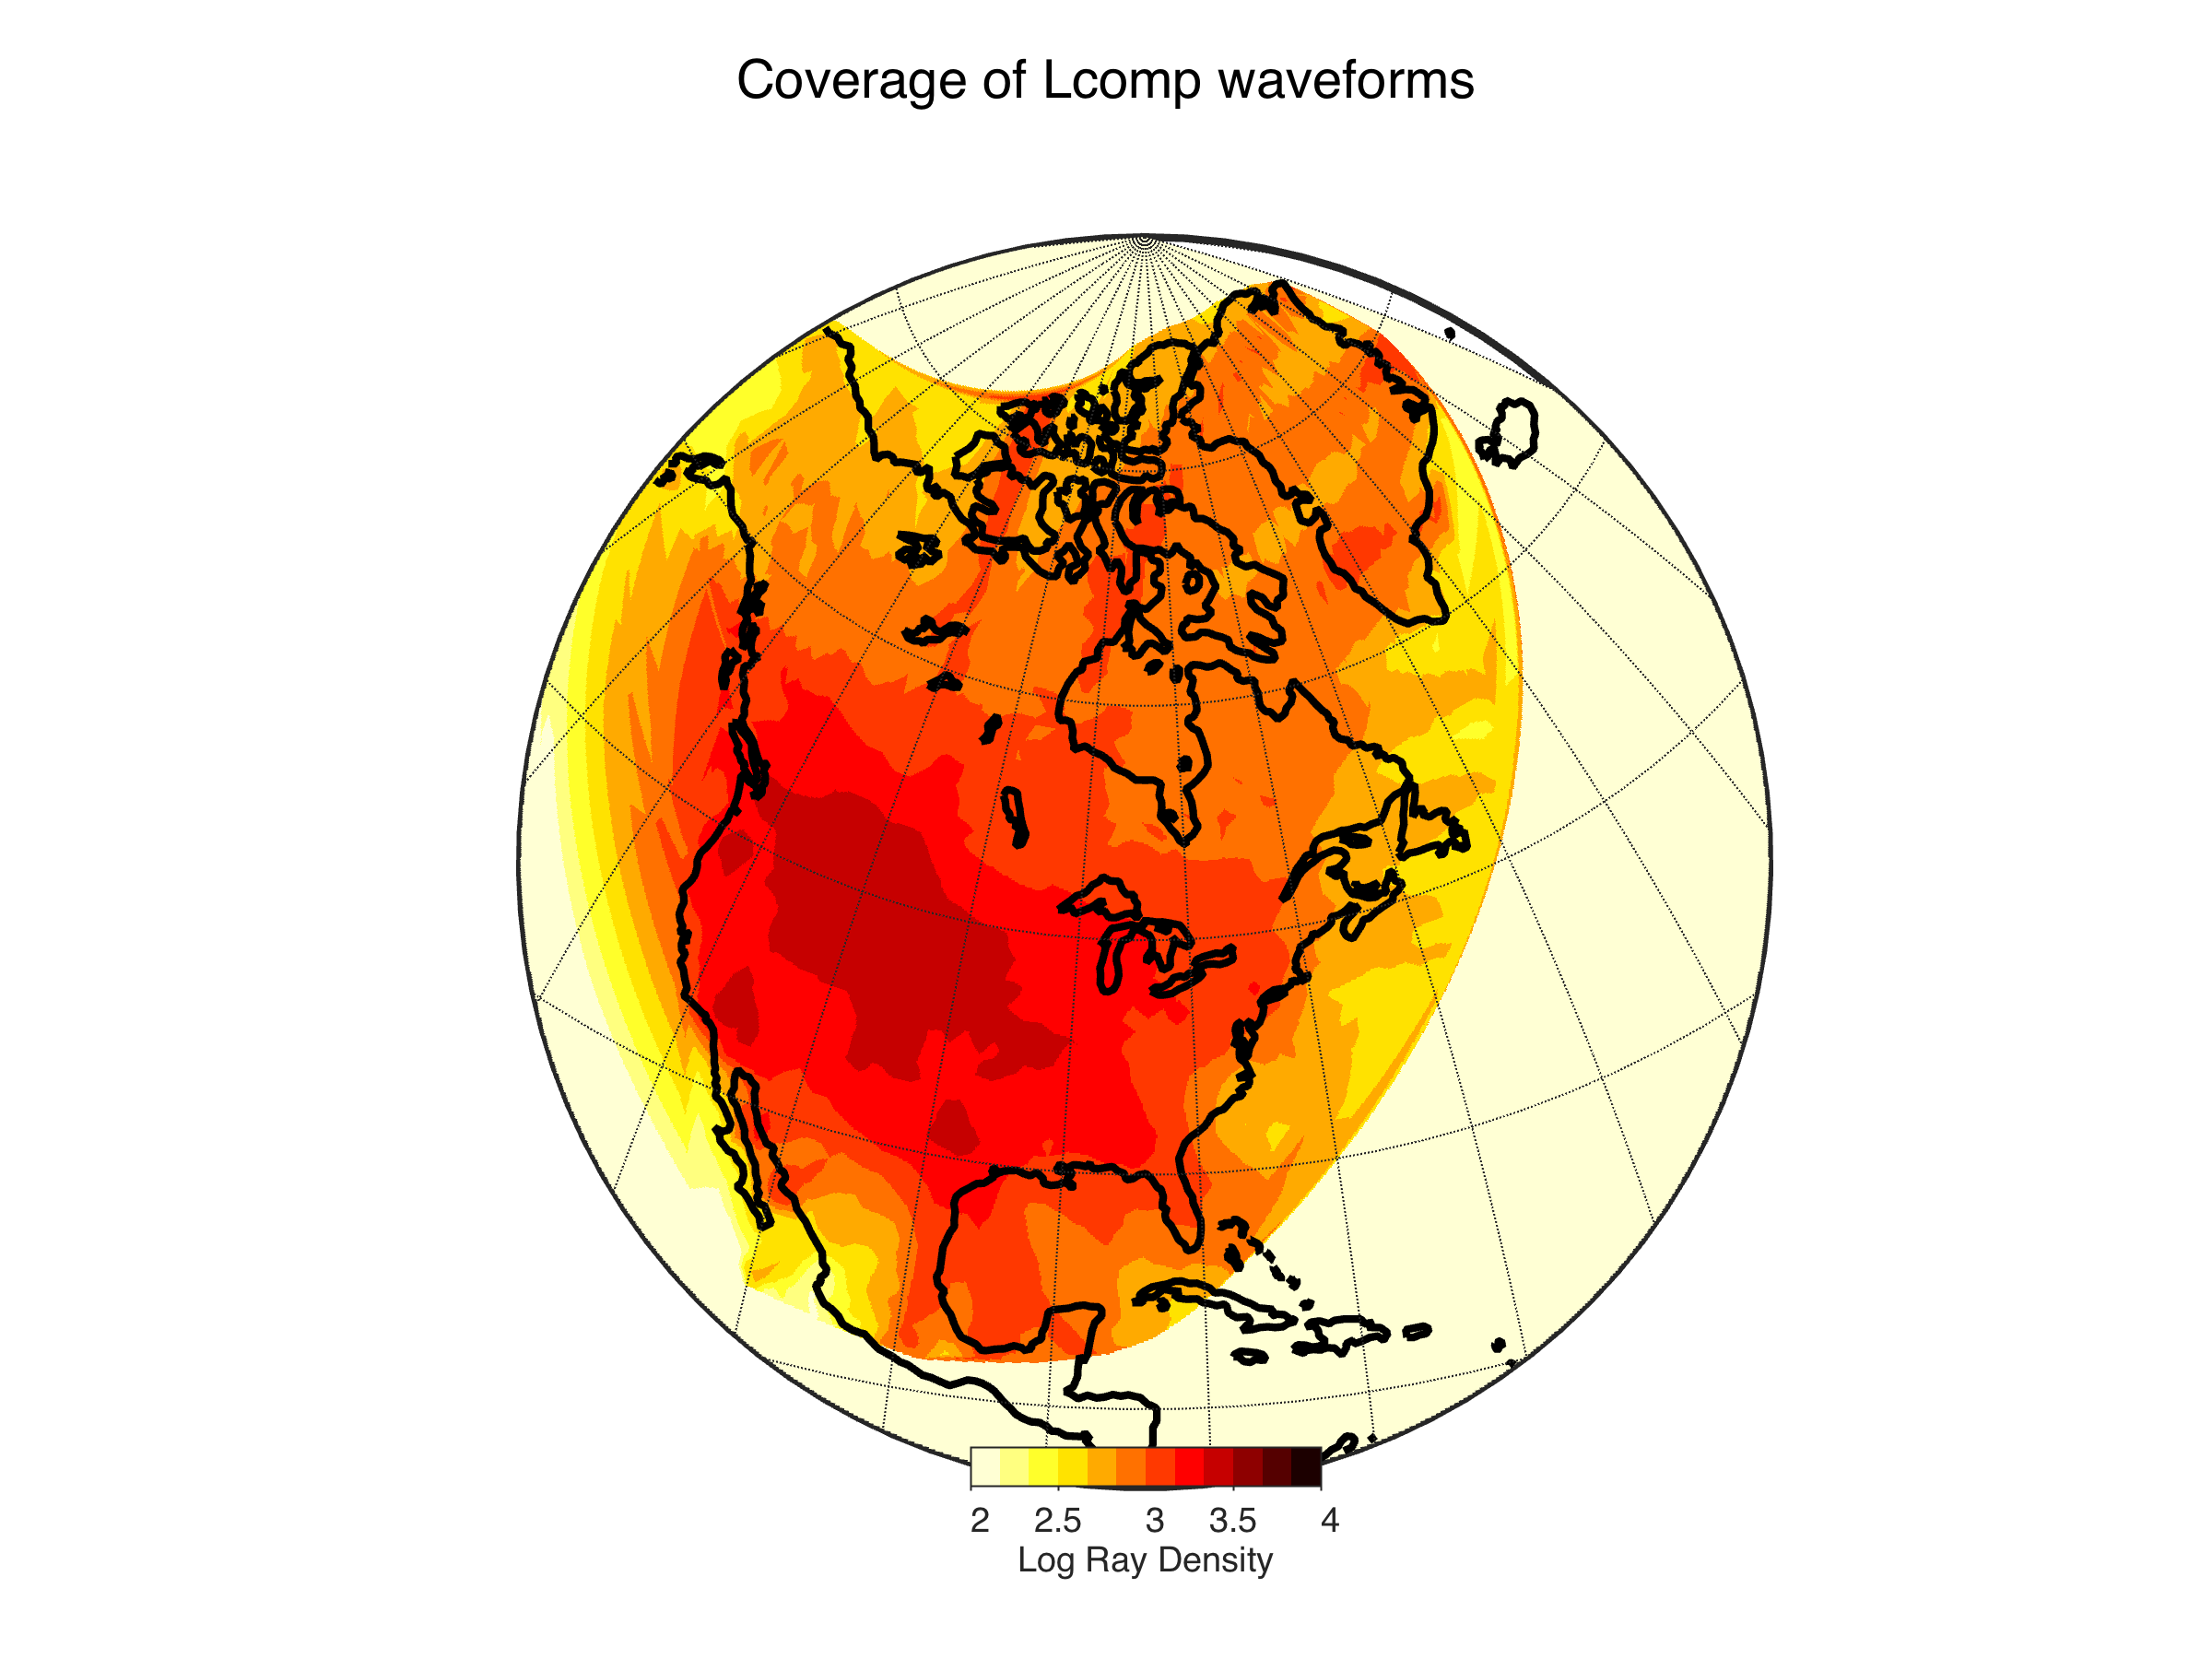
\includegraphics[viewport=120 10 470 420,clip=,width=\linewidth]{figures/Coverage_L_iter3.png}}
	\end{minipage}
	\hfill
	\begin{minipage}{0.47\linewidth}
		\centerline{\includegraphics[viewport=120 10 470 420,clip=,width=\linewidth]{figures/Coverage_T_iter3.png}}
	\end{minipage}

	\begin{minipage}{0.47\linewidth}
		\centerline{\includegraphics[viewport=120 10 470 420,clip=,width=\linewidth]{figures/Coverage_Z_iter3.png}}
	\end{minipage}
	\hfill
	\begin{minipage}{0.47\linewidth}
		\centerline{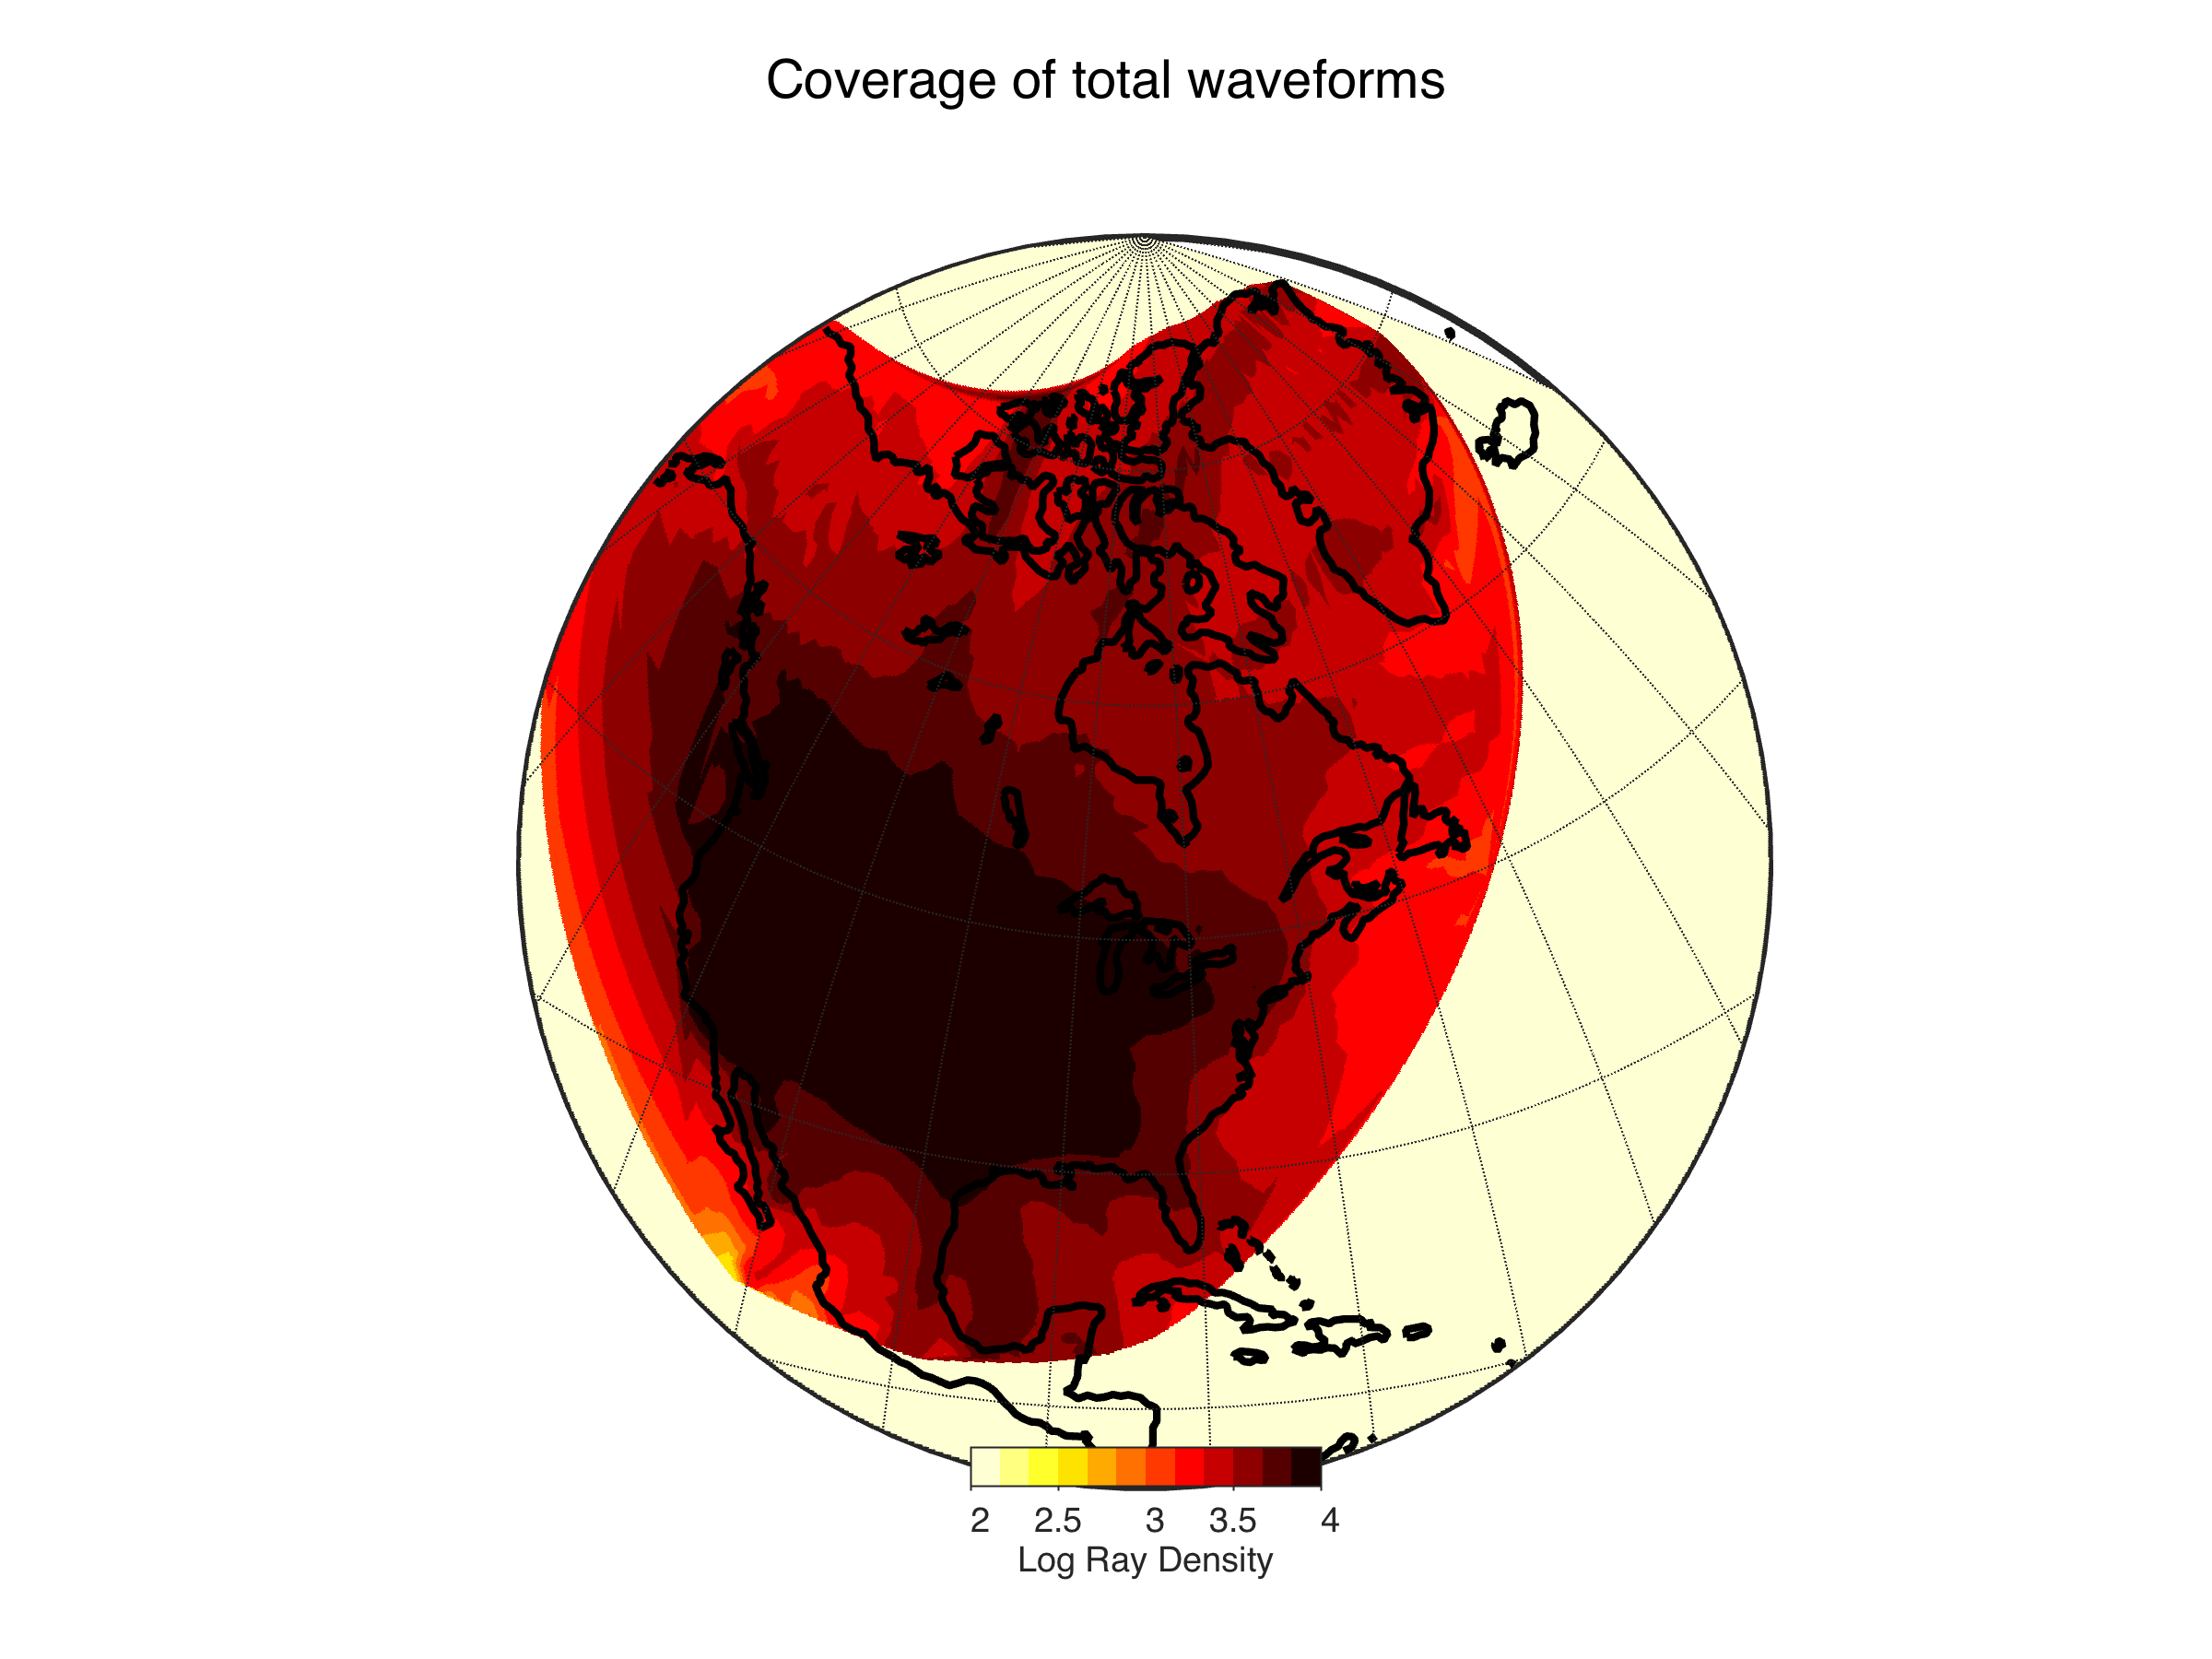
\includegraphics[viewport=120 10 470 420,clip=,width=\linewidth]{figures/Coverage_all_iter3.png}}
	\end{minipage}

\caption{Density coverage for each component and all gathered.} 
\label{density_coverage}

\end{figure}


In addition to long period waveforms, we also consider a group velocity dispersion dataset \citep{shapiro2002monte} provided in the form of $1^o \times 1^o $ maps between 25 and 100 s. 
The shorter periods (below 60 s) are used to constrain our homogeneized crustal structure at each iteration, as described below, while the entire period range is included during the inversion for mantle structure, providing additional constraints for structure in the shallow parts of the mantle, that are consistent with the treatment of the crust.

As in our previous work at the global scale \citep{french2013waveform,french2014whole}, we do not rely on an existing layered crustal model. 
There are several drawbacks to considering such models. 
First, they are constructed using data for limited regions that are then extrapolated to other regions based on a tectonic regionalization, and may not always fit real waveform data very well. 
Second, the inclusion of thin low velocity layers slows down the SEM computation significantly. 
Instead, we compute a radially anisotropic smooth crustal model on a $2^o \times 2^o $ grid through Monte Carlo Markov Chain (MCMC) simulation constrained by the group velocity dispersion data. 

This process is called "homogeneization" \citep[e.g.][]{backus1962long,capdeville2008shallow}, and yields a crustal model equivalent to a real crust within the period range of the data used to constrain it (i.e. here for periods longer than 20s). 
The thickness of the crust is a priori fixed to that of model Crust2.0 \citep{basscrust2} when it is larger or equal to 30 km, and it is fixed at 30 km in regions where it is thinner. 
This results in a smooth, but realistic crust within most of the continent, and a crustal model that is not directly interpretable in the border regions of our model space (i.e. in the oceans and borders of the continent where the real crust is thin). 
We have shown that this does not bias the mantle structure imaged below 50 km \citep{french2014whole}. 
At each iteration of the inversion, we only invert for structure below 30 km depth, and subsequently recompute the crustal model for the next iteration by applying our MCMC approach with mantle structure fixed to that of the current iteration model. 
The procedure is described and discussed in detail in \cite{french2014whole}

Assuming that our azimuthal coverage is everywhere sufficient within our target region, we here solve only for radially anisotropic structure. If (A,C,F,L and N) are the 5 elastic parameters describing a radially anisotropic (or VTI) medium \citep{love2013treatise}, then:

\begin{equation}
 N = \rho V^{2}_{SH}, \quad L = \rho V^{2}_{SV}, \quad A = \rho V^{2}_{PH} , \quad C = \rho V^{2}_{PV} 
 \end{equation}
then the medium can equivalently be described by the 5 parameters ($V_{S}, V_{P}, \xi, \phi, \varepsilon$) where:

\begin{equation}
V_{S} = \sqrt{\frac{2V^{2}_{SV}+V^{2}_{SH}} {3}} \\
V_{P} = \sqrt{\frac{V^{2}_{PV} + 4V^{2}_{PH}}{5}}
 \xi = \frac{N}{L}, \quad \varphi = \frac{C}{A}, \quad \eta = \frac{F}{A-2L} 
 \end{equation}

We only consider two of the 5 independent anisotropic parameters , those to which long period surface waveforms are the most sensitive: isotropic velocity $V_{S}$ and the anisotropic parameter $\xi = {\frac{V_{SH}}{V_{SV}}}^2$, where $V_{SH}$ is the velocity of waves polarized horizontally and $V_{SV}$ that of waves polarized vertically . 
The other three parameters and density are constrained through empirical scaling relationships, following \cite{montagner1989petrological}, and are based on laboratory measurements for upper mantle rocks. 

The scaling parameters considered are \citep{montagner1989petrological}

 \begin{equation}
\frac{\delta(V_{P})}{\delta(V_{S})} = 0.5, \quad
\frac{\delta(\rho)}{\delta(V_{S})} = 0.33, \quad
\frac{\delta(\eta)}{\delta(\xi)} = -2.5,   \quad
\frac{\delta(\varphi)}{\delta(\xi)} = -1.5,   \quad
\end{equation}

We chose a parametrization in terms of $V_S$ and $\xi$, rather than $V_{SH}$ and $V_{SV}$, as this allows us to consider different spatial resolution and apply higher damping in the inversion to the less well resolved anisotropic parameter $\xi$, rather than having to reconstruct this parameter from differences in perturbations in the two quantities $V_{SH}$ and $V_{SV}$, which would limit the resolution allowed in isotropic velocity.

In previous studies \citep{marone2007depth,yuan2010lithospheric}, after inverting for radial anisotropic structure \citep{marone2007three,yuan20113}, we also inverted for azimuthal anisotropy, by adding constraints from SKS splitting measurements. This step will be the topic of a separate publication.  

The target model space is geographically defined as shown in Figure ~\ref{map_evt_stn}, and is limited in depth down to 800 km. 
As in our previous tomographic studies, the model space is parametrized in terms of 26 cubic splines $\nu_{q}(r)$ vertically \citep{megnin2000three} from the core-mantle boundary to 30 km deep. 
Although we invert for structure only in the top 16 splines, corresponding to the top 700-800 km of the mantle. 
The spline nodes are spaced more closely at shallow depths, and located at the following radii: 5690, 5810, 5910, 5900, 6061, 6101, 6131, 6161, 6191, 6221, 6241, 6261, 6281, 6301, 6321, 6341 km.  
Laterally, we parametrize our model in terms of spherical splines $\beta(\theta,\phi)_{p}$ \citep{wang1995spherical}. 
The combination of vertical and spherical splines constitutes a local basis for the description of smooth functions within the model volume. 
Thus, the value of a model parameter $m(r,\theta,\phi)$ can be computed at any point in space given the set of spline coefficients $m_{pq}$:

\begin{equation}
	m(\theta,\varphi,r) = \sum_{p}\sum_{q}m_{pq}\beta_{p}(\theta,\varphi)\nu_{q}(r)
\end{equation}

The spherical spline parametrization has the advantage of allowing for variable grid parametrization, which can be adjusted according to data coverage \citep[e.g.][]{marone2007three}. 
In our case, outside of the target region, we adopt a "level 6" spherical grid for $V_{S}$ ($2^{o}$ knot spacing) and a "level 4" spherical grid for $\xi$ ($8^{o}$ knot spacing), consistent with the parametrization of $SEMUCB\_wm1$ \citep{french2014whole}. 
Inside the well-sampled target region, we define a level 7 spherical grid ($1^{o}$ knot spacing) for $V_{S}$ and level 6 ($2^{o}$ knot spacing) for $\xi$. 

 \subsection{Forward modelling}

\begin{figure}[p]
% \centering
	\begin{tabular}{ccc}
		(a)&&(b)\\
		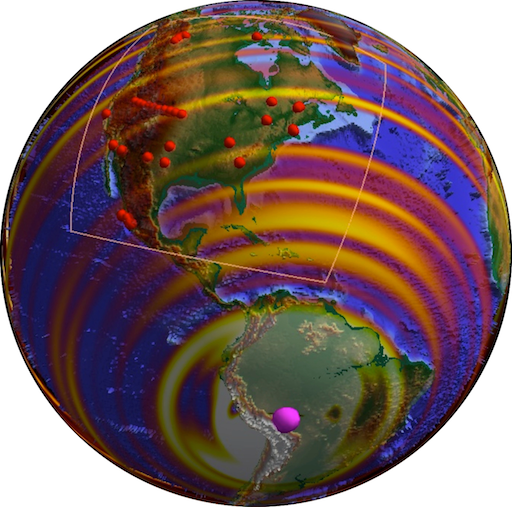
\includegraphics[width=.4\textwidth]{figures/snap_glob.pdf} && 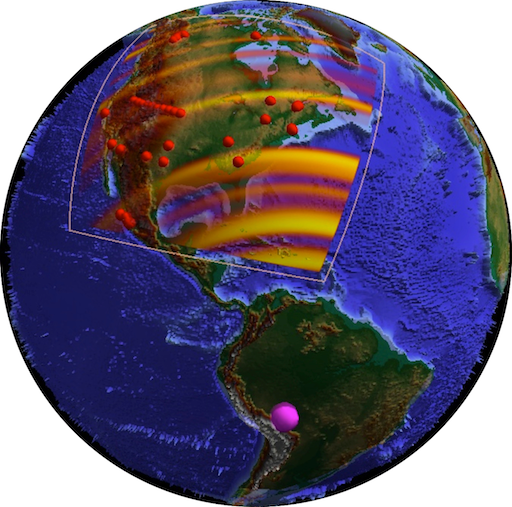
\includegraphics[width=.4\textwidth]{figures/snap_reg.pdf} \\ 
		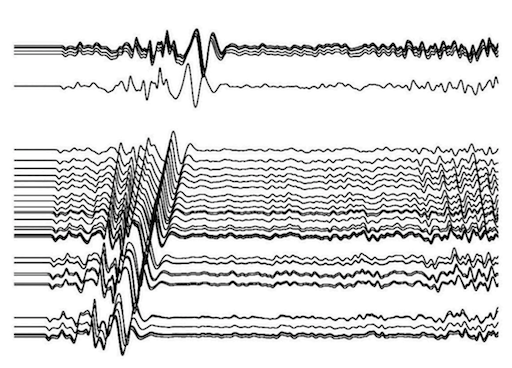
\includegraphics[width=.4\textwidth]{figures/seismo.pdf}    && 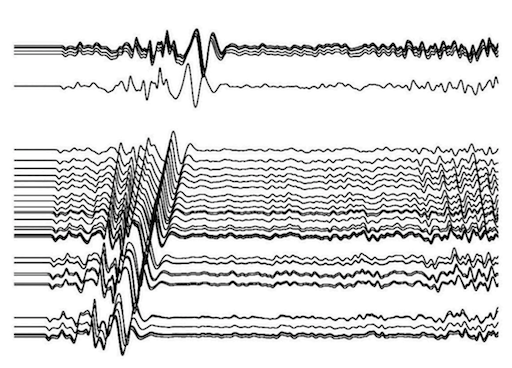
\includegraphics[width=.4\textwidth]{figures/seismo.pdf}
	\end{tabular}

	\caption{\baselineskip 18pt 
		Comparison between a global scale simulation and a regional scale simulation of wave propagation following an earthquake in south America. The seismograms corresponds to the recordings at 37 station located in north America (red spheres).
		The pink sphere shows the epicenter of the earthquake. In (a), the wavefield is modeled globally using the spectral element method Specfem3D\_globe \citep{komatitsch2002spectrala}. In (b), the wavefield is modeled regionally using the RegSEM. During the inversion, all the synthetic seismograms are computed using the regional SEM code RegSEM \citep{cupillard2012regsem} code and regenerated thanks to virtual sources located around the computational domain \citep[see][]{masson2013numerical}. The sismograms in (b) are exactly similar to those in (a), however, the computational effort is greatly reduced in the regional simulation (b).}

	\label{injection}

\end{figure}

During the inversion, all the synthetic seismograms are computed using the regional SEM code RegSEM \citep{cupillard2012regsem} that takes into account effects of oceans, topography/bathymetry, ellipticity, and anelasticity, and where the limits of the computational domain (white box around North America in Figure~\ref{injection} and red box in Figure ~\ref{map_evt_stn}) are dealt with using absorbing boundaries. 
The synthetic seismograms associated with regional data (i.e. where both the seismic stations and the earthquake are located within the regional modeling domain) do not require any specific treatment and are computed as in our previous studies using RegSEM \citep[e.g.][]{yuan2014lithospheric}. 
The synthetic seismograms associated with teleseismic data (i.e. where the earthquake and the seismic stations are located outside and inside the regional modeling domain, respectively) are obtained using a two step procedure as proposed by \cite{masson2016box} as follows. 

Prior to the inversion, the wavefields generated by teleseismic earthquakes are computed globally within our starting model ($SEMucb\_wm1$) and a version of $SPECFEM3D\_globe$ \citep{komatitsch2002spectrala} adapted to this model representation. 
During these global simulations, the 3 component displacement wavefield is recorded at a set of points with locations prescribed by the RegSEM code.
Within the regional solver RegSEM, these points are the collocation or Gauss-Lobatto-Legendre (GLL) points belonging to the one element thick surface surrounding the regional modeling domain \citep[see][]{masson2013numerical}. 
Note that our procedure does not require to store either the stress or the strain wavefield, which are computed naturally by the regional solver. This makes it easy to swap between different codes for modeling global seismic wave propagation (i.e. any code that outputs displacement seismograms can be used as such).
Because the Courant criteria which ensure the stability in SEM often lead to oversampling, we compress the recordings versus time using a least square B-spline transform \citep{unser1993a,unser1993b}. We found this  approach more efficient and practical than the more classic decimation/interpolation scheme.
We typically achieve a data compression ratio of between 10 and 100 with no significant loss of accuracy. 
During the inversion, the global recordings are transformed to virtual sources that regenerate the global wavefield regionally. 
This operation is done on the fly by the RegSEM code.

Overall, the additional computational effort to account for teleseismic events consists of one global simulation per teleseismic event. These simulations are done once and for all before the inversion starts. A comparison between regular $SPECFEM3D\_globe$ and ``RegSEM + virtual sources`` synthetics is shown in Figure~\ref{injection}.

\subsection{Inverse modelling}

In continuity of our previous work \citep[e.g][]{marone2007three,yuan20113,yuan2014lithospheric}, we use a hybrid iterative inversion scheme where, at each iteration, the forward wavefield is computed accurately using SEM, but the inverse step is solved using the formalism of \cite{tarantola1982generalized} with sensitivity kernels calculated approximately using normal mode perturbation theory. 
This allows us to apply a fast converging Gauss-Newton quadratic optimization scheme. 
As shown in \cite{tarantola2005inverse}, and in Appendix A of \cite{lekic2011inferring}, it is far more important to use an accurate forward modelling scheme to compute the misfit function, provided of course that the theory captures the effects of the background long wavelength structure accurately \citep[unlike the examples shown in][]{valentine2016impact}.
Inaccuracies in the theoretical treatment of kernels then result in smoothing errors that can be compensated for in subsequent iterations. In contrast, currently popular "adjoint tomographic" approaches \citep{zhu2015seismic,bozdag2016global} compute the numerically exact gradient, however, they also need to apply smoothing operators and regularization, which degrades the accuracy of their kernels. Importantly, they rely on a linear optimization scheme (conjugate gradient method), which is characterized by very slow convergence.

Our misfit function is defined in the time domain from the point by point differences between observed and synthetic waveforms as follows:
\begin{equation}
2\Phi(m_{k}) = [d - g(m_{k})]^{T} C^{-1}_{d} [d-g(m_{k})] + [m_{p}-m_{k}]^{T} C_{m}^{-1} [m_{p}-m_{k}]
\end{equation}

\noindent where $m_{k}$ represents the model estimate at the k-th iteration, $d$ is the data vector (waveform discretized in time or group velocity as a function of period) and $g(m_k)$ is the corresponding discretized wavefield computed using SEM, or the predicted group velocity dispersion. The model prior is $m_p$  (i.e. the 3D starting model) and $C_m$ and $C_d$ represent a priori model and data covariance matrices, respectively. Minimizing $\Phi$ in the sense of the L2 norm leads to the equation for the k+1 model update:

\begin{equation}
m_{k+1} = m_{k} + (C_{m}G^{T}_{k}C^{-1}_{d}G_{k} + I)^{-1} (C_{m}G_{k}^{T}C^{-1}[d-g(m_{k})]+ m_{p}-m_{k})
\end{equation}

\noindent where $G$ is the matrix of Frechet derivatives of $g(m)$ calculated at $m_k$. We compute G using NACT or PAVA, depending on the distance range of the corresponding source-station path.
NACT and PAVA are both asymptotic (high frequency) approximations to first order normal mode perturbation theory. 
The PAVA includes along branch mode coupling only and is equivalent to the standard surface wave approximation \citep[e.g][]{mochizuki1986free,romanowicz1987multiplet}, as used for example in \cite{woodhouse1984mapping}, in which a frequency shift and distance shift are introduced for each mode to account for the effects of heterogeneous structure. 
The corresponding kernels are "1D", i.e. they only depend on the average structure between the source and the receiver. This approximation is valid for single-mode seismograms, such as fundamental mode surface waves \citep[e.g][]{romanowicz2008computation}.
NACT includes across branch-coupling, in addition to PAVA, which brings out 2D sensitivity of waveforms in the vertical plane containing the source and the receiver. NACT breaks down when the distance between the source and station is short, so we compute kernels using NACT for epicentral distances larger than $15^o$, and PAVA for shorter distances.
Neither PAVA nor NACT consider off-great circle plane sensitivity (i.e. focusing effects, e.g. \cite{zhou2005finite}). These effects become important for accurate amplitude fitting. With our choice of misfit function, we are first and foremost fitting the phase, and for that, the 2D effects in the vertical plane are dominant, and important especially for overtones, as illustrated in \cite{megnin1999effects,romanowicz2008computation}.


\section{Results}

\begin{figure}[ht]
	\centering
	\includegraphics[width=1\textwidth]{figures/Vs-60-300-for-paper.png}

	\caption{\baselineskip 18pt
	3D isotropic shear wave velocity structure of the continent. Map views are shown from 60 km down to 300 km, shown as variations with respect to the regional mean (thick red line in Figure ~\ref{1daverage}). 
	% Labels are: BP, Blake Plateau; NQ, New Quebec Orogen; THO, Trans-Hudson Orogen. State abbreviations are: CO, Colorado; MT, Montana; ND, North Dakota; SD, South Dakota; and WY, Wyoming. 
	% The geological limits of the cratonic crust are indicated as follows: (to be defined when using final figures... 
	}

	\label{3d-VS}

\end{figure}

\begin{figure}[ht]
	\centering
	\includegraphics[width=1\textwidth]{figures/Xi-60-300-for-paper.png}

	\caption{\baselineskip 18pt
	3D isotropic radial anisotropy structure of the continent. Map views are shown from 60 km down to 300 km, shown as variations with respect to the regional mean (thick red line in Figure ~\ref{1daverage}). 
	% Labels are: BP, Blake Plateau; NQ, New Quebec Orogen; THO, Trans-Hudson Orogen. State abbreviations are: CO, Colorado; MT, Montana; ND, North Dakota; SD, South Dakota; and WY, Wyoming. 
	% The geological limits of the cratonic crust are indicated as follows: (to be defined when using final figures... 
	}

	\label{3d-Xi}

\end{figure}


The tomographic inversion results for $V_S$ and $\xi$ are presented in figures \ref{3d-VS} and \ref{3d-Xi} respectvely. 
We divide the model description and interpretation into two parts, focusing first on the continent-wide structure and then, in more detail, on eastern different regions.

\subsection{Continental model}
\begin{figure}[ht]
	\centering
	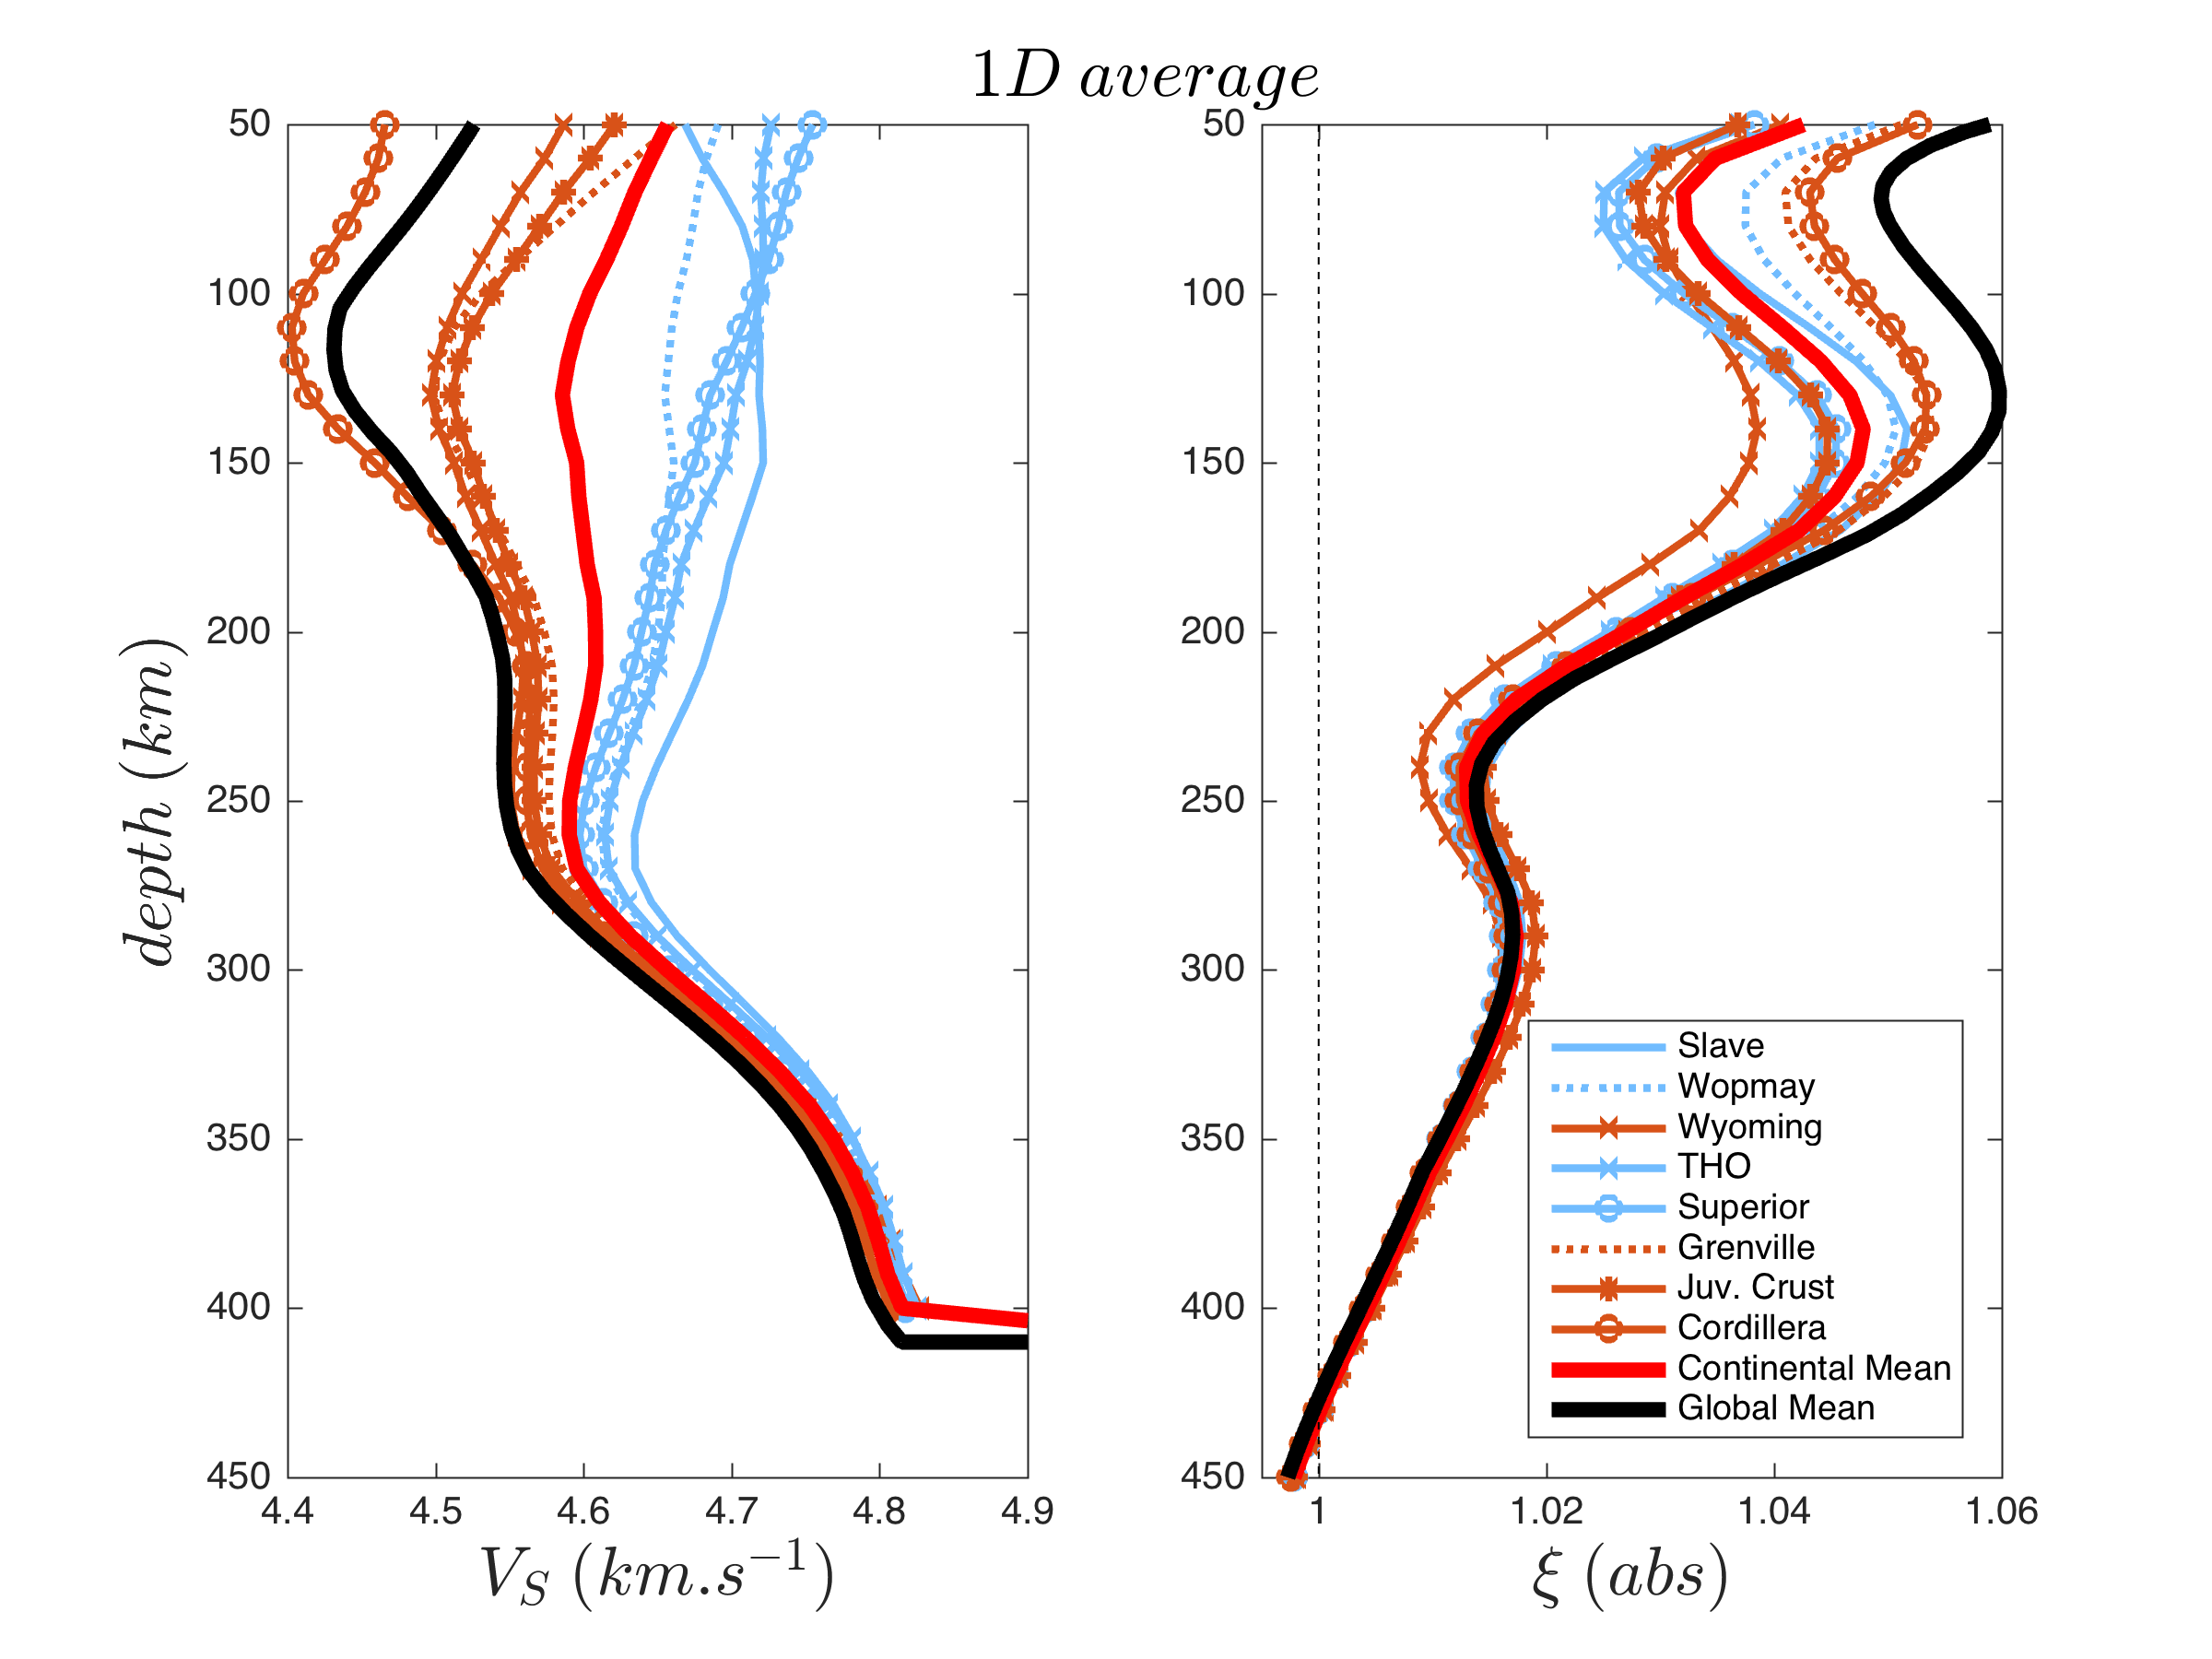
\includegraphics[width=1\textwidth]{figures/1D_profile_with_regions.png}

	\caption{\baselineskip 18pt 
	1D average depth profiles for isotropic shear velocity (left) and radial anisotropy (right), for the SEMucb\_wm1 global model (thick black), the continental average (thick red); and depth profiles for different regions in the model (see legend and Figure~\ref{mapgeol}). The continental average is always higher than the global average in terms of $V_S$, while for $\xi$, they are similar deeper than $250 \: km$.}
	\label{1daverage}
\end{figure}

As observed in many other studies, the average isotropic shear velocity $V_S$ in the shallow upper mantle beneath North America (NA) is high compared to the global average, which contains contributions from large oceanic regions (Figure ~\ref{1daverage}). 
The difference persists until ca. $270 \: km$ depth and then fades away, though, $V_S$ remains slightly higher in NA than in the global average. 
Compared to the continental average, precambrian provinces like Wyoming, Yavapai, Mazatzal, Great Rhyolites and Grenville are caracterized by slower velocities. 
The cordillera region shows the slowest velocities, close the global average as for $\xi$. 
Closer to the center of the continent, region like Slave, T.H.O, Juvenile arcs and orogens (e.g. Wopmay), Superior; show higher velocities with the Slave province caracterized by a positive gradient above $100 \: km$ deep.

%The global negative gradient of $V_S$ near $150km$ is here less pronounced beneath the continent by the influence of the positive gradient beneath the cratonic part. (I don't think we need stress this -discussing differences between east and west will be more interesting.

The average of $\xi$ is higher than $1$ (which means that $V_{SH} > V_{SV}$), but lower than the global average, the latter influenced by the strong $\xi > 1$ oceanic signature.
% where shearing is more important. 
Both trends are similar with depth, but the maximum in $\xi$ is slightly deeper than in the global average and the change from $V_{SH} > V_{SV}$ to $V_{SH} < V_{SV}$ is reached at ca. $420km$. 

{\color{red} This feature was already present in the global model, and perturbations below that depth are <1\% So I dont think the model adds more informations compared to SEMucb}.

I am on this part..

\subsection{Beneath the craton}

\begin{figure}
	\begin{minipage}{0.5\linewidth}
		\centerline{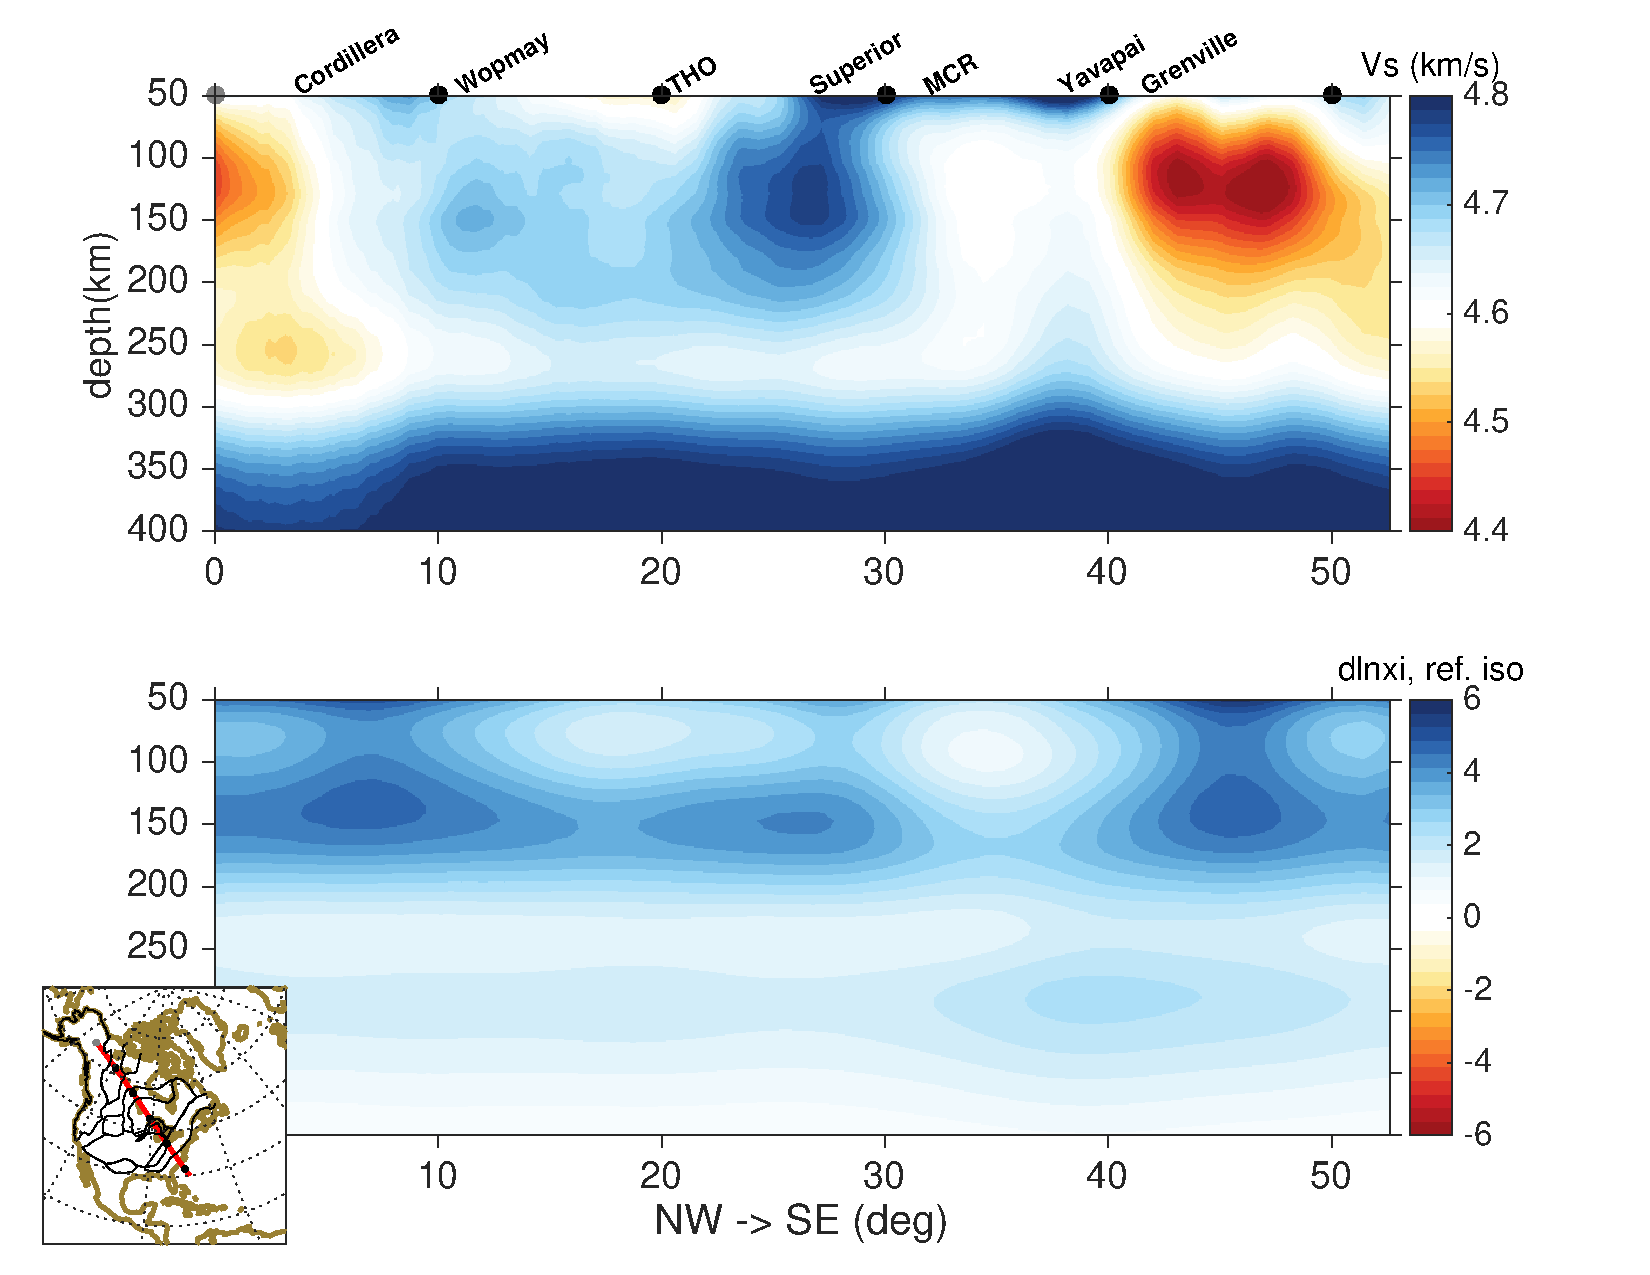
\includegraphics[width=\linewidth]{figures/profiles_NASEM3_vs_dxi_A.pdf}}
	\end{minipage}
	\hfill
	\begin{minipage}{0.5\linewidth}
		\centerline{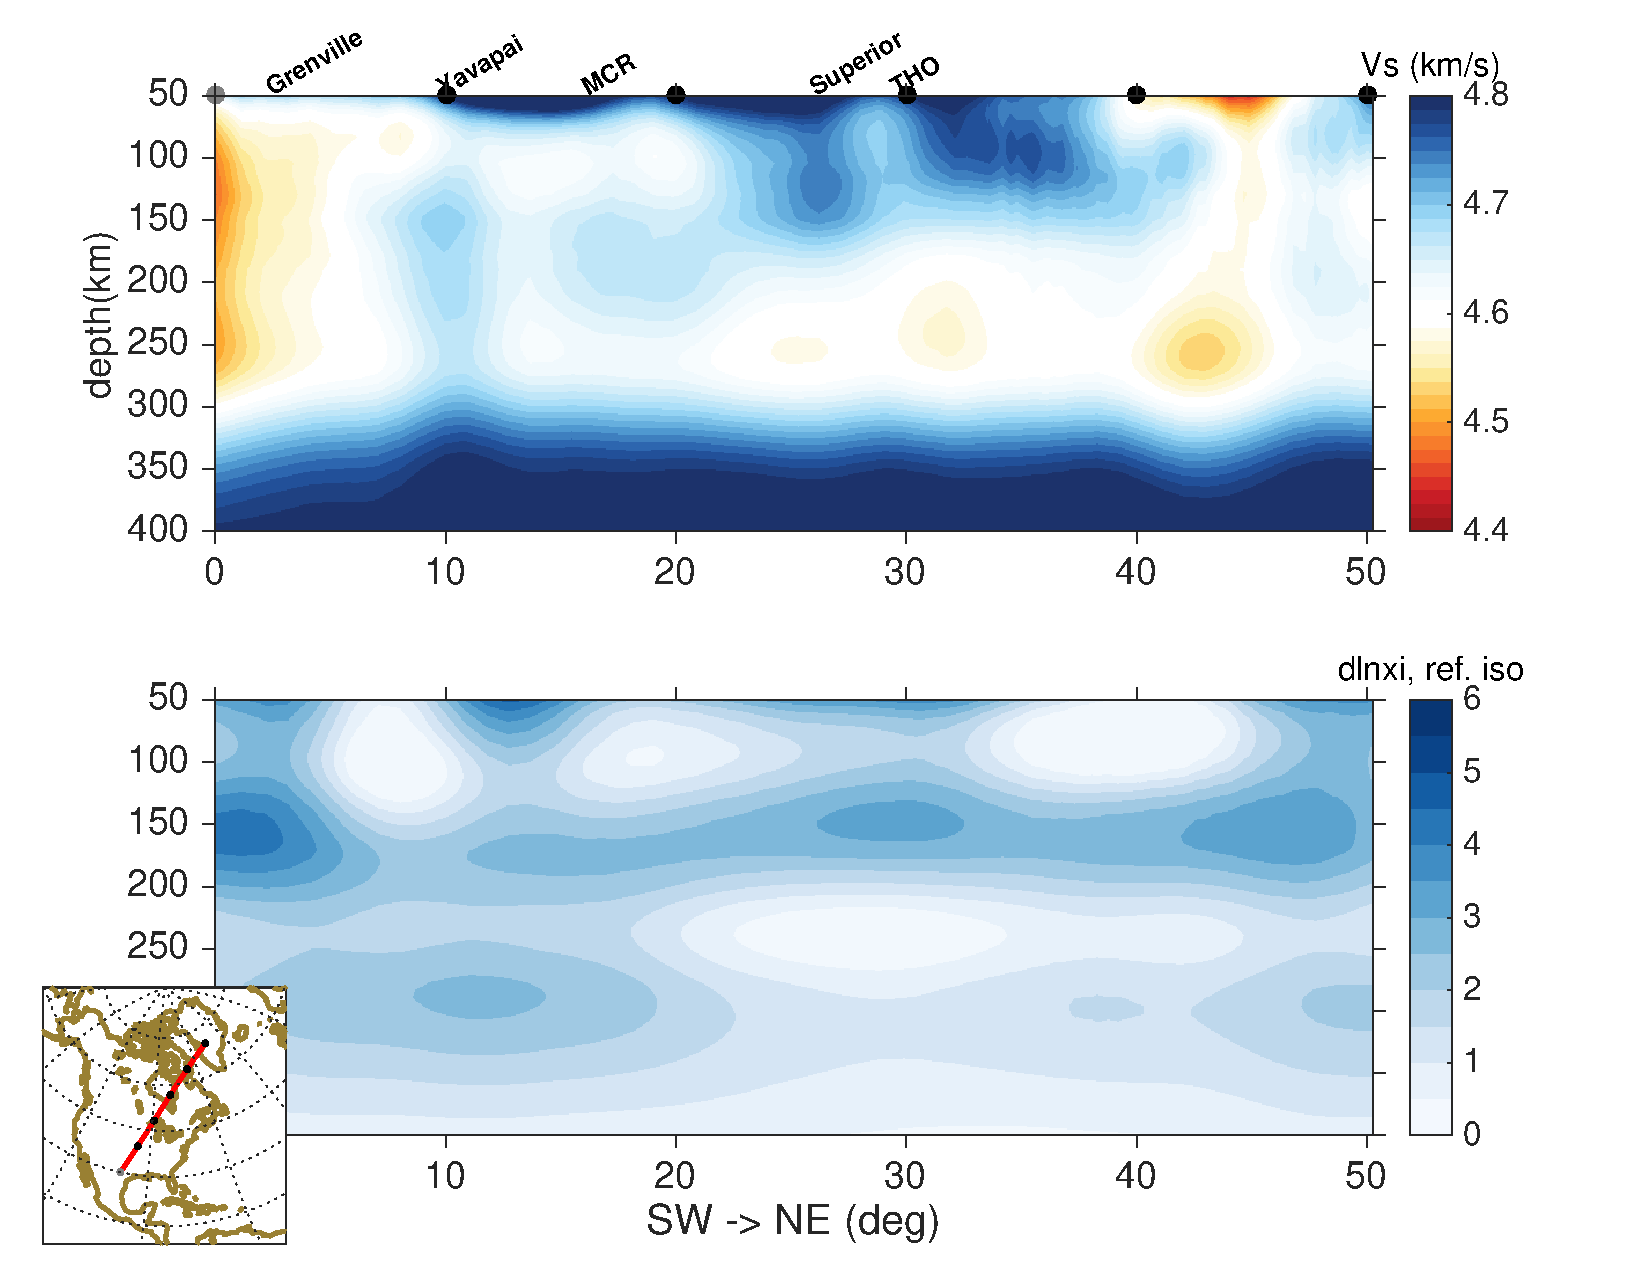
\includegraphics[width=\linewidth]{figures/profiles_NASEM3_vs_dxi_B.pdf}}
	\end{minipage}

	\caption{Cross Section of the lithospheric core}
	\label{cratoncross}

\end{figure}

% Gung 2003 Positive anomalies of dlnxi down to 400km in the craton.

Our study confirms the presence of a thick lithospheric root in the craton with faster than average $V_S$ down to $250km$ depth, with highest velocities, ca. $4.8km.s^{-1}$, located at depths shallower than  $150km$ (e.g. Figure~\ref{cratoncross}). 
Laterally, the cratonic root in $V_S$ coincides roughly with precambrian aged crust (see Figure~\ref{3d-VS} from 60 to 150km deep)
The western edge of the craton follows the RMF (black thick dashed line in Figure \ref{mapgeol}), instead of the western breakup line (See the red thin line in Figure~\ref{mapgeol} which coincides with RMF in Canada, but is diverging westward in the U.S.). While the eastern/south-esatern coincides with the Llano-Grenville Front (See the blue thin line in Figure~\ref{mapgeol}). 
The northern part ends at the coastline of the Arctic ocean including the arctic archipelago and Greenland. 


\begin{figure}
	\begin{minipage}{0.5\linewidth}
		\centerline{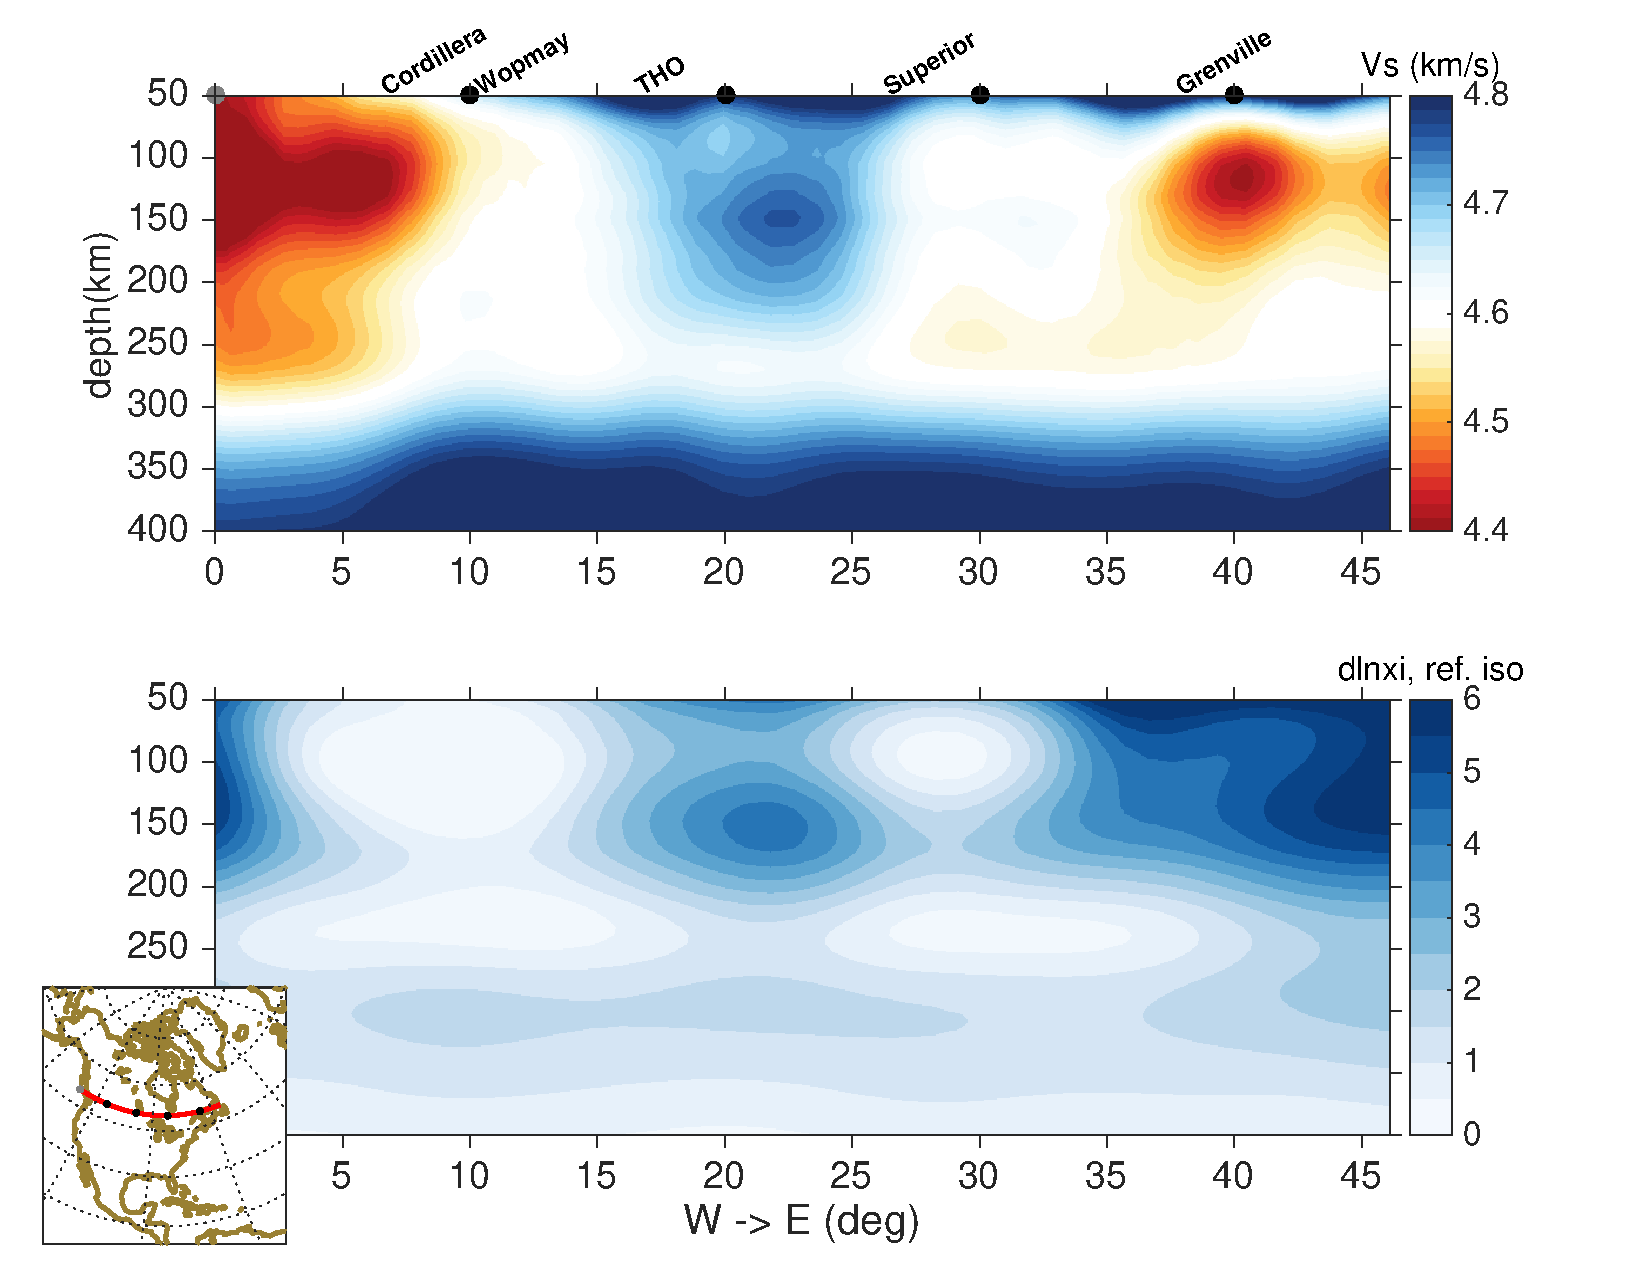
\includegraphics[width=\linewidth]{figures/profiles_WE-50.pdf}}
	\end{minipage}
	\hfill
	\begin{minipage}{0.5\linewidth}
		\centerline{\includegraphics[width=\linewidth]{figures/profiles_SN-100.pdf}}
	\end{minipage}

	\caption{Cross Section of the lithospheric core showing the core retraction}
	\label{cratoncrossedge}

\end{figure}

These lateral edges are well observed down to $150km$ depth. Below that, the cratonic root retracts toward the center of the archaean continent and is still present beneath Slave, Hearne/Rae and western Superior cratons as shown in Figure \ref{cratoncrossedge}. 
Everywhere within the craton, a negative gradient of $V_S$ is observed, marking the base of the lithosphere, with a minimum of $\sim 4.6km.s^{-1}$ reached at $\sim 300km$ depth. 
While the base of the lithosphere (and top of the low velocity zone- LVZ) shows strong topography, the bottom of the LVZ appears largely flat, in particular under the  Slave, Hearne/Rae and western Superior cratons.

As observed in \cite{babuvska1998age,gung2003global,yuan2014lithospheric}, there are large lateral variations  $\xi$ down to $\sim 200km$ depth, with regions of reduced radial anisotropy, in contrast to the more uniform, positive $dln(\xi)$ structure in this depth range in the oceans (See figure \ref{3d-Xi}. 
Below 250km, it is interesting to note that there is a large band of positive anomaly crossing the whole continent (across the US), making the connection between the Pacific and Atlantic mantles.

Generally, $\xi$ always appear higher than 1. 
Except around 100 km, negative absolute values of $\xi$ (lower than -$1\%$) are observed in Mexico, at the southern part of Florida, the southern part of the Superior craton comprising the Mid Continental rifting, the southern part of the Granit Rhyiolite Province comprising the Failed Rifting area and finally beneath Baffin Island. 


\subsubsection{Wyoming}{h}
% \begin{figure}
% 	\begin{minipage}{0.5\linewidth}
% 		\centerline{\includegraphics[width=\linewidth]{figures/profiles_NASEM3_vs_dxi_wyoming_A.pdf}}
% 	\end{minipage}
% 	\hfill
% 	\begin{minipage}{0.5\linewidth}
% 		\centerline{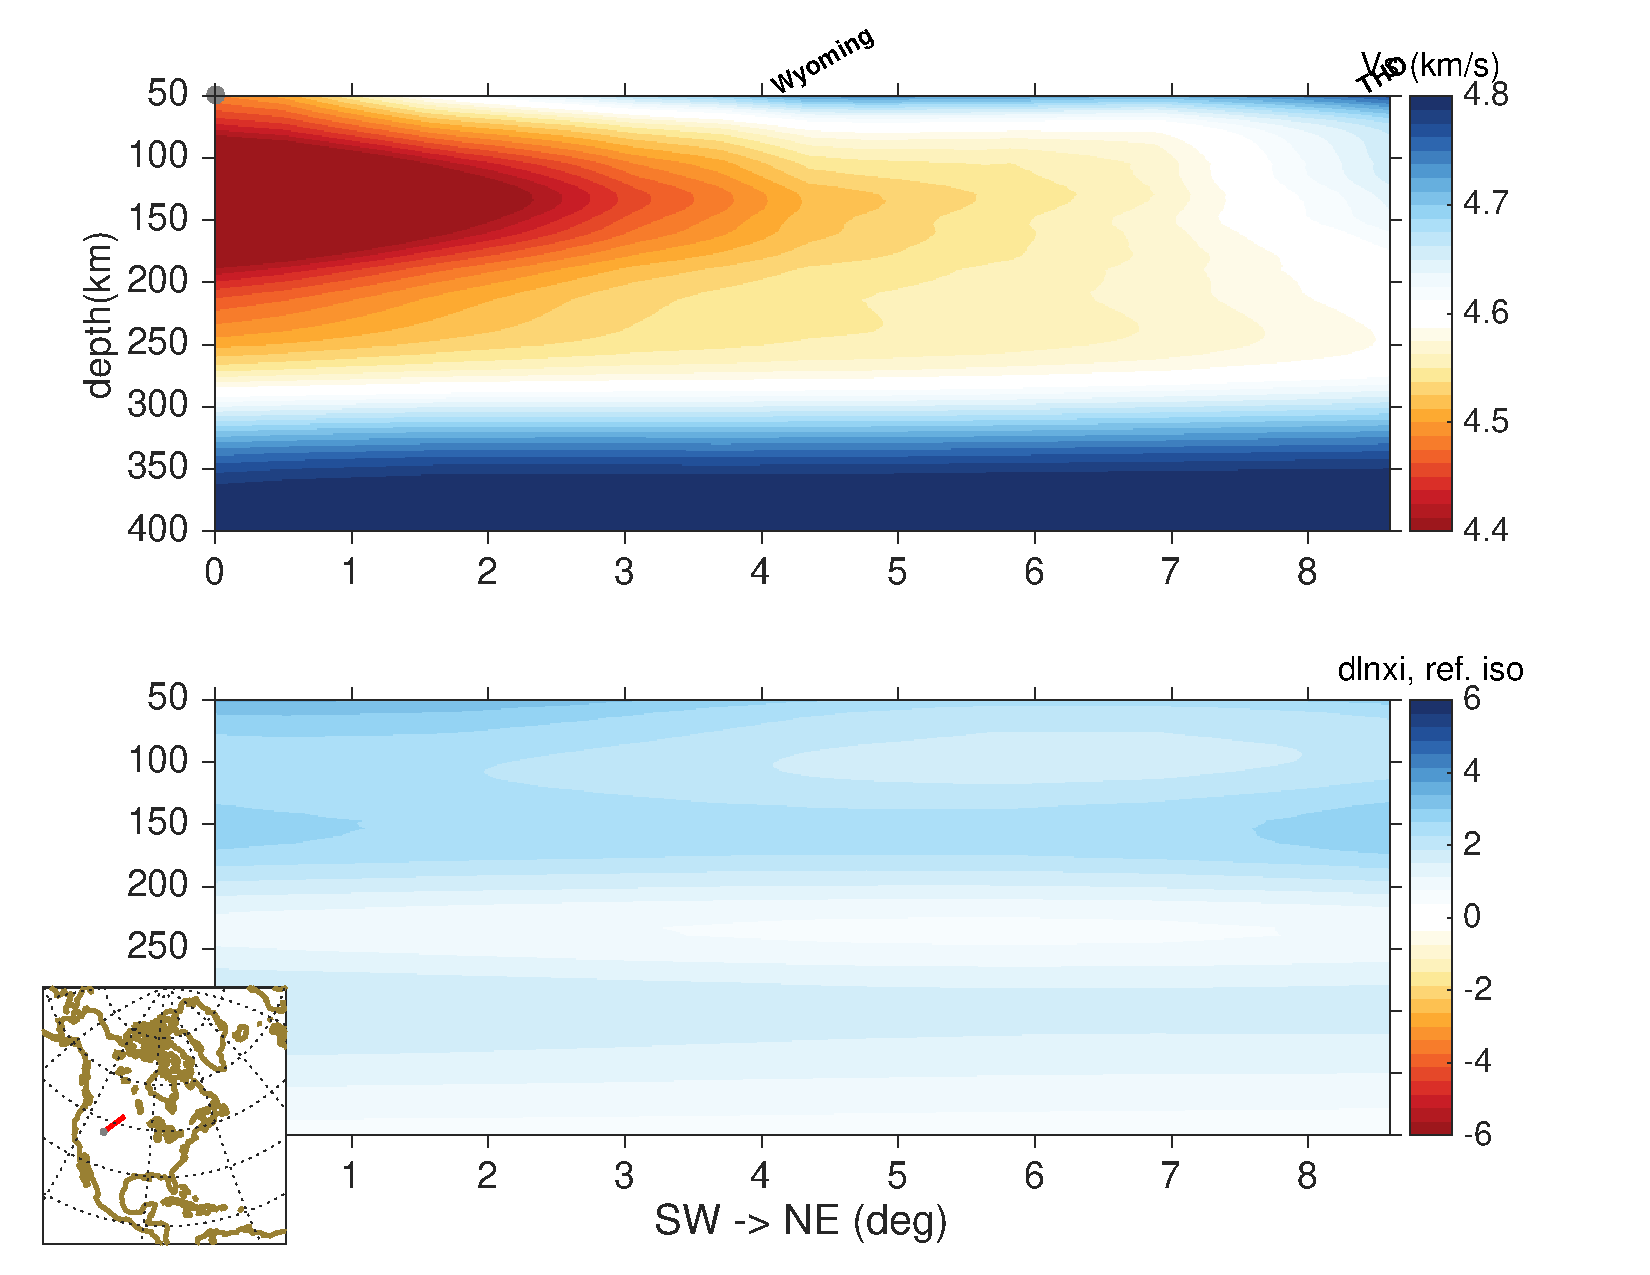
\includegraphics[width=\linewidth]{figures/profiles_NASEM3_vs_dxi_wyoming_B.pdf}}
% 	\end{minipage}

% 	\caption{Cross Section of the Wyoming lithosphere}
% 	\label{wyomingcross}

% \end{figure}

The Archaean aged Wyoming craton does not show as high anomalies as within the craton nucleus as shown in figure ~\ref{3d-VS}. 
It is split into 2 distinctive part. A western part showing low velocities influenced by the active tectonic with a radially positive gradient. 
In contrast with the eastern part showing higher velocities with a radially negative then positive gradient. 
The depth of negative gradient's minima is variable, from 70 (western part) to 250km (eastern part) deep. 
The separation between the two areas coincides with the RMF.

\subsubsection{Slave}

	% \begin{figure}
	% 	\begin{minipage}{0.5\linewidth}
	% 		\centerline{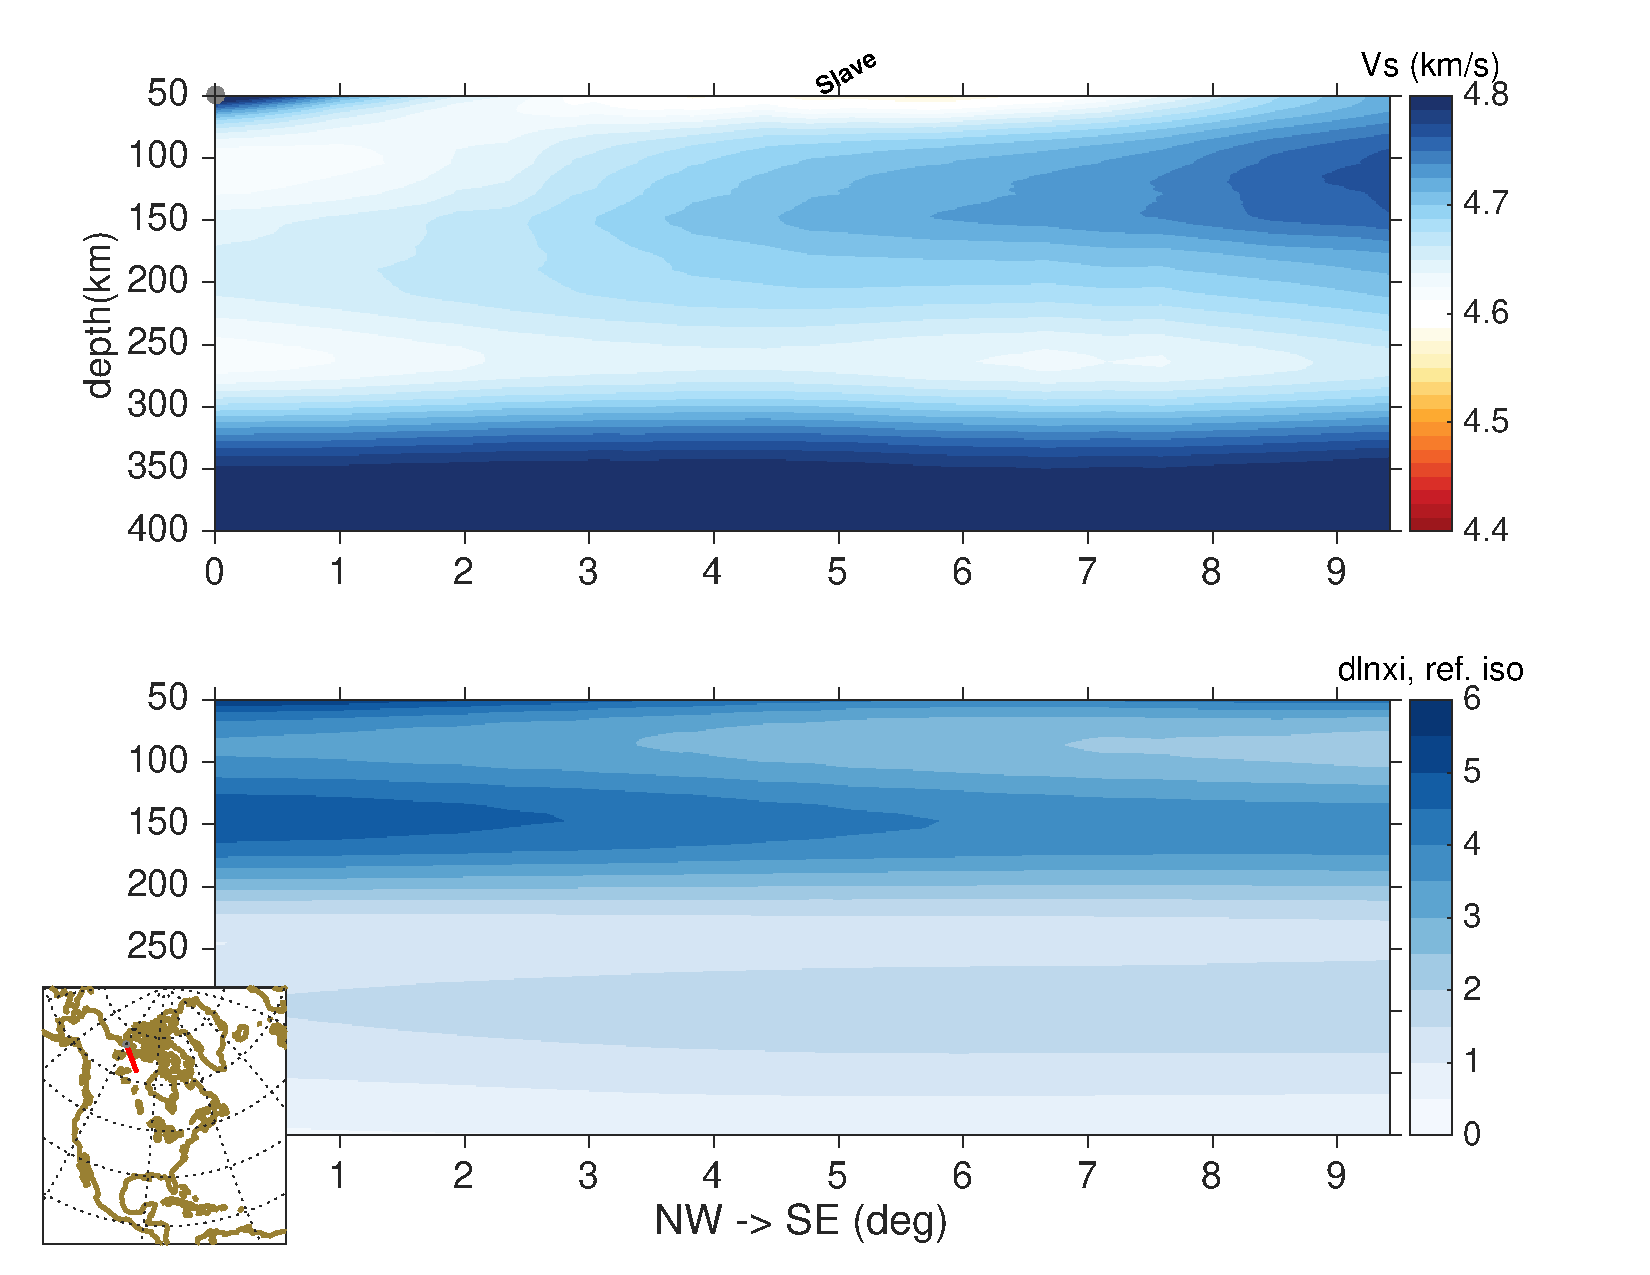
\includegraphics[width=\linewidth]{figures/profiles_NASEM3_vs_dxi_slave_A.pdf}}
	% 	\end{minipage}
	% 	\hfill
	% 	\begin{minipage}{0.5\linewidth}
	% 		\centerline{\includegraphics[width=\linewidth]{figures/profiles_NASEM3_vs_dxi_slave_B.pdf}}
	% 	\end{minipage}

	% 	\caption{Cross Section of the Slave lithosphere}
	% 	\label{slavecross}

	% \end{figure}

	The Archaean aged Slave craton shows typical lithospheric craton signatures with higher than average velocities as shown in figure ~\ref{3d-VS} and in figure~\ref{cratoncross}. 
	It shows in the entire region a positive velocity gradient with a maximum of ca. $4.8km.s^{-1}$ associated with a maximum of $\xi$ at ca. $150km$ deep.
	Deeper, a negative gradient is observed with a minimum of ca. $4.6km.s^{-1}$ at ca. $250km$ deep. 
	The topography of the extrema appears flat. (Est ce que c'est une characteristique d'un craton stable non deforme?)
	Although the Slave lithosphere shows highest velocities at $150km$, above $100km$ velocities are slightly higher than the continental average ($dln(V_S)< 4\%$).

\subsubsection{Superior Craton}
	In our model, the Superior craton can be split in two parts: The western part showing typical cratonic structures while the eastern part shows slower velocities at all depths. Below $150km$, velocity anomalies are below $2\%$ (almost $0\%$). 

	\paragraph{Western part}
		% \begin{figure}
		% 	\begin{minipage}{0.5\linewidth}
		% 		\centerline{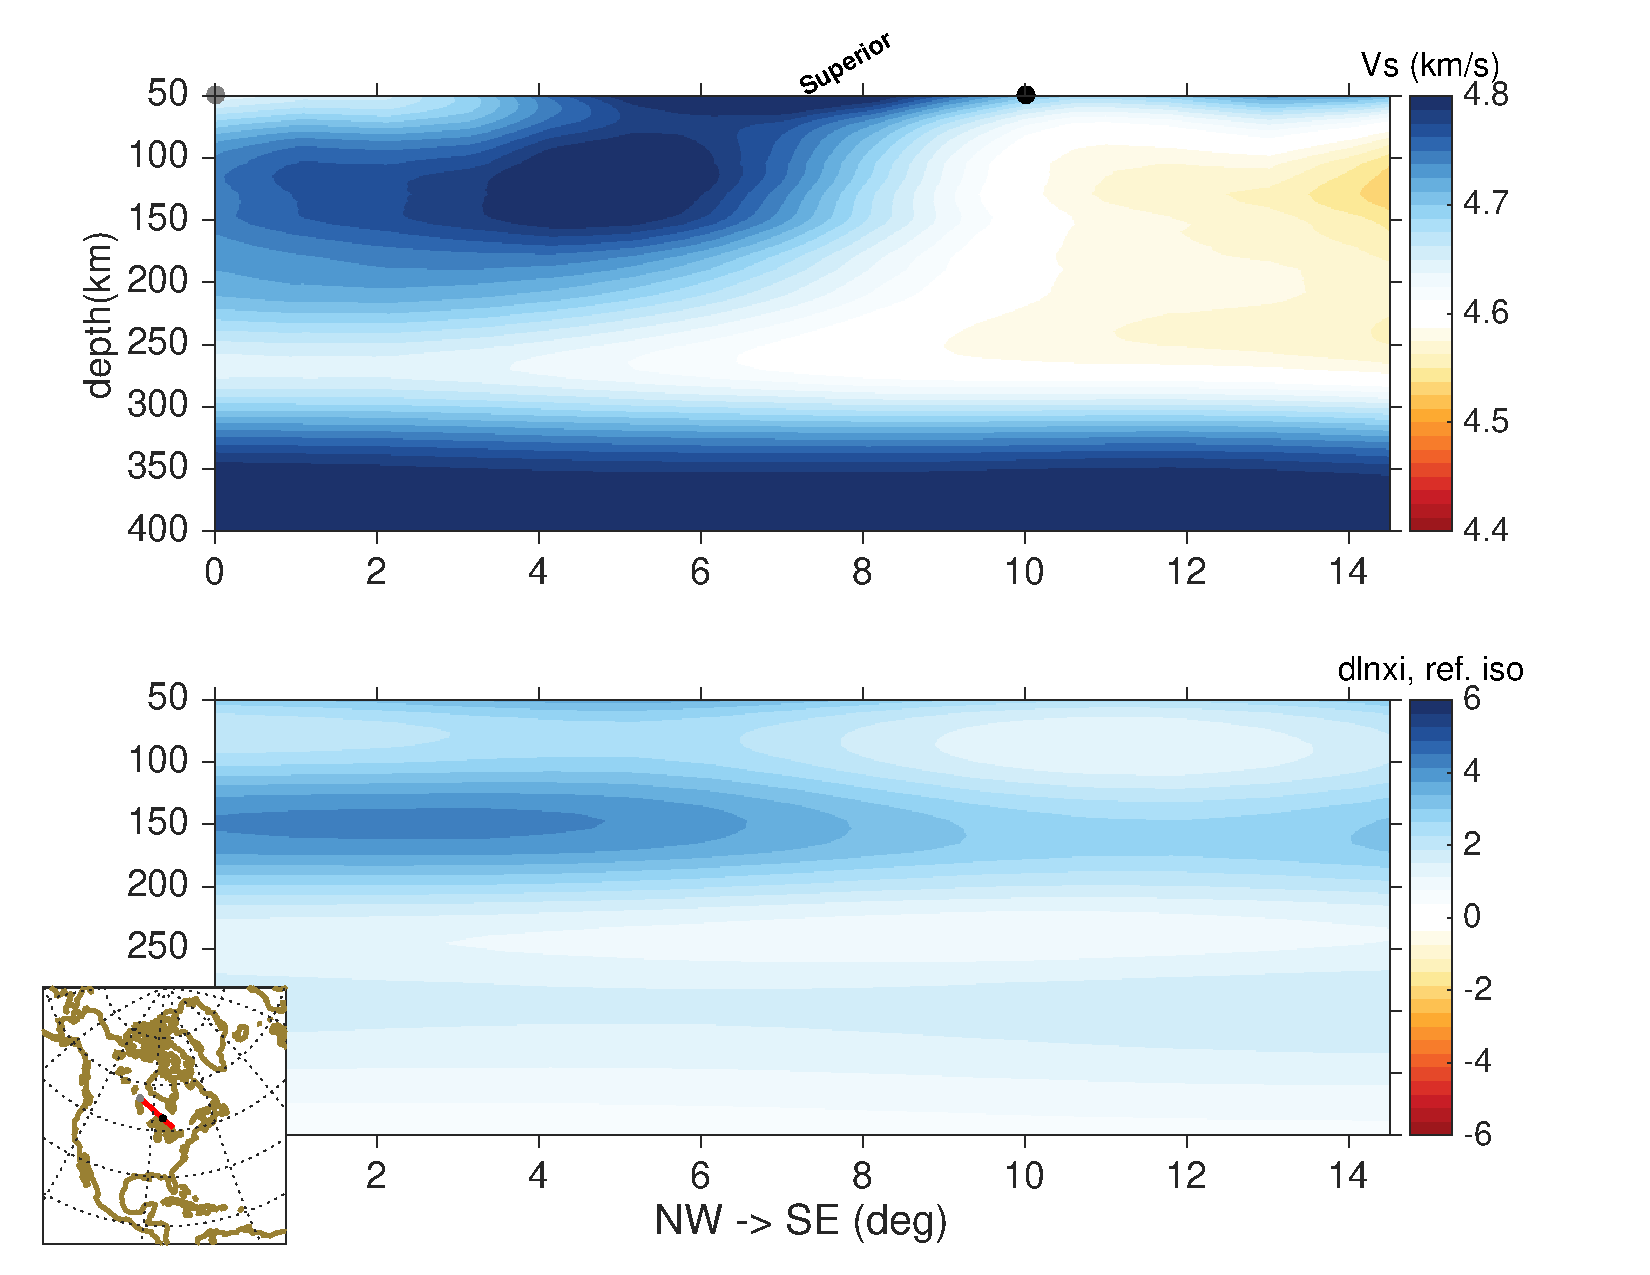
\includegraphics[width=\linewidth]{figures/profiles_NASEM3_vs_dxi_west_superior_A.pdf}}
		% 	\end{minipage}
		% 	\hfill
		% 	\begin{minipage}{0.5\linewidth}
		% 		\centerline{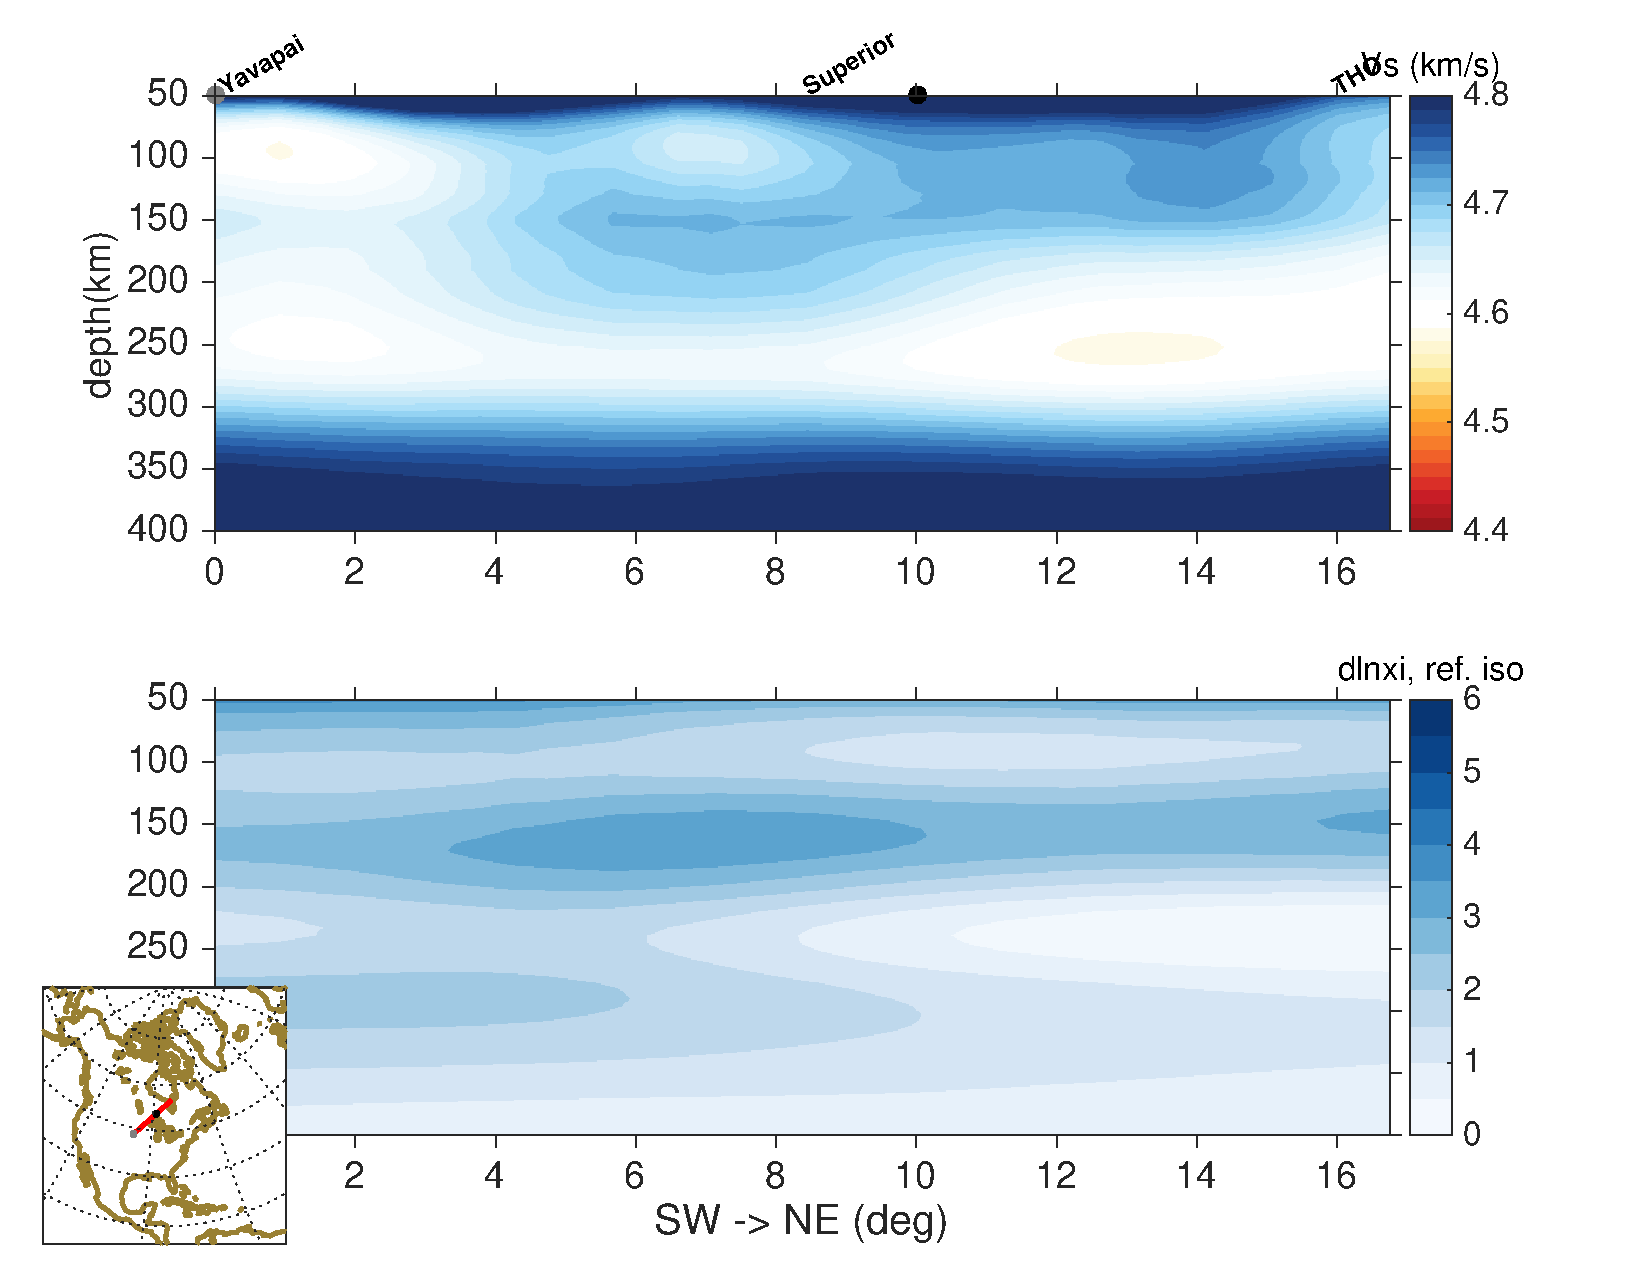
\includegraphics[width=\linewidth]{figures/profiles_NASEM3_vs_dxi_west_superior_B.pdf}}
		% 	\end{minipage}

		% 	\caption{Cross Section of the western Superior lithosphere}
		% 	\label{westsupcross}

		% \end{figure}

		The Archaean aged Superior craton shows typical lithospheric craton signatures with higher than average velocities as shown in figure ~\ref{3d-VS} and in figure~\ref{cratoncross}. 
		It shows in the entire region a positive velocity gradient with a maximum of ca. $4.8km.s^{-1}$  associated with a maximum of $\xi$ at ca. $150km$ deep.

		Deeper a negative gradient is observed with a minimum of ca. $4.6km.s^{-1}$ at ca. $250km$ deep. 
		Opposed to the Slave craton, the topography of the extrema is variable. 
		From SW to NE, the core of maximum velocity can reach beween 70 and 150km of thickness. 
		Beneath the maximum velocity region of ca. $150km$ the negative gradient appears stipper than beneath the $70km$ one, while the topography of the deeper positive gradient appears flat. 
		At the south-eastern part of the western Superior, close the Mid-Lithospheric rift, we can observe the thinning of the cratonic lithosphere when crossing the Grenville front. 
		The band of minimum velocity within the cratonic root has similar amplitudes, in terms of velocity, than beneath the younger lithosphere but at shalower depths between $100$ and $150km$. 
		Following the Great Meteor track built by \cite{heaman2000timing}, which crosses the Superior craton, it is interseting to note that the low velocity channel beneath the base of the lithosphere shows lower velocties than usualy observed beneath the other Archaean cratons. 
		This slow anomaly corresponds to the V-shape dent, or divot, observed by \cite{lee1997upper} who explained the feature by the presence of water in the mantle. 
		We observe at $250km$ that the slow anomaly go further inland and crosses the Superior Craton northward until the Hudson bay following the GMT.

		\paragraph{Eastern part}
		% \begin{figure}
		% 	\begin{minipage}{0.5\linewidth}
		% 		\centerline{\includegraphics[width=\linewidth]{figures/profiles_NASEM3_vs_dxi_east_superior_A.pdf}}
		% 	\end{minipage}
		% 	\hfill
		% 	\begin{minipage}{0.5\linewidth}
		% 		\centerline{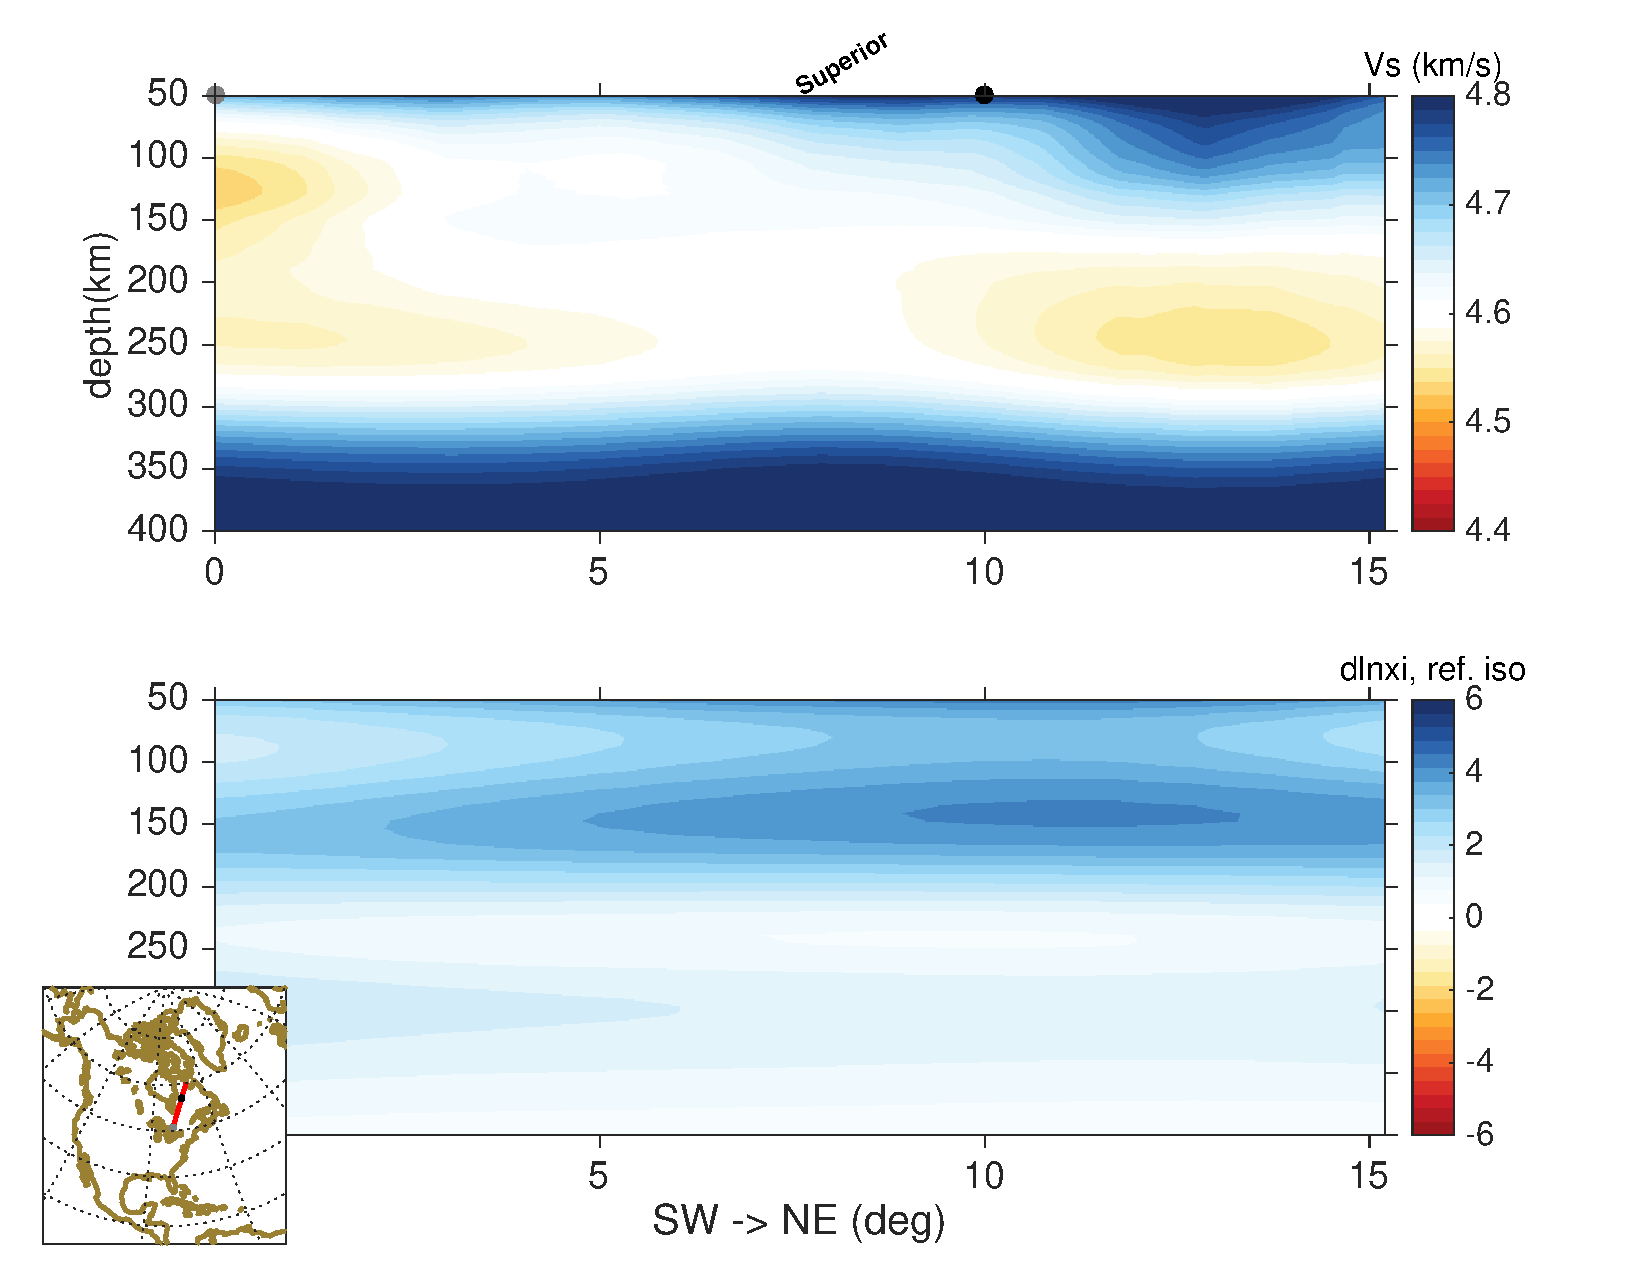
\includegraphics[width=\linewidth]{figures/profiles_NASEM3_vs_dxi_east_superior_B.pdf}}
		% 	\end{minipage}

		% 	\caption{Cross Section of the western Superior lithosphere}
		% 	\label{eastsupcross}

		% \end{figure}

		Compared to its western part, the structure here shows differences as shown in figure ~\ref{cratoncrossedge} 
		Fast velocities are present down to $150km$deep but are slower. 
		The negative gradient is steeper and the minimum is radially thicker. 
		However at the center, the minimum channel is not continuous and shows higher (still slower than the center of the western Superior) velocities.
		% the gradual trend in velocity is replaced by an almost constant slow anomaly from $150$ to $300km$ deep.   

\subsubsection{Trans Hudson Orogen}
	The Trans Hudson Orogen (THO) is a belt of Paleo-Proterozoic aged region. It refers to a major tectonic event (between $2.0$ to $1.8Ga$) that welded Archaean blocks to form the Laurentia Craton.
	% At shallow depths ($ < 60km$) shows lower velocities than archaean surroundings. 
	It is interesting to notice that at shallower depths than $100km$, the proterozoic THO (including the Sask craton) which welded the Superior and Rae/Hearne cratons, shows lighter (i.e, $+4\%$ compared to $+8\%$) positive anomalies than its archaean surrounding. While most of the proterozoic root start to thin out at $150km$, the THO at the vicinity of the hudson bay shows as high anomalies as Rae/Hearne and Superior areas. 
	Je suis en train de construire des profils le long de THO pour voir!

\subsubsection{Yavapai/Mazatzal/Granit-Rhyolite region}
	% \begin{figure}
	% 	\begin{minipage}{0.5\linewidth}
	% 		\centerline{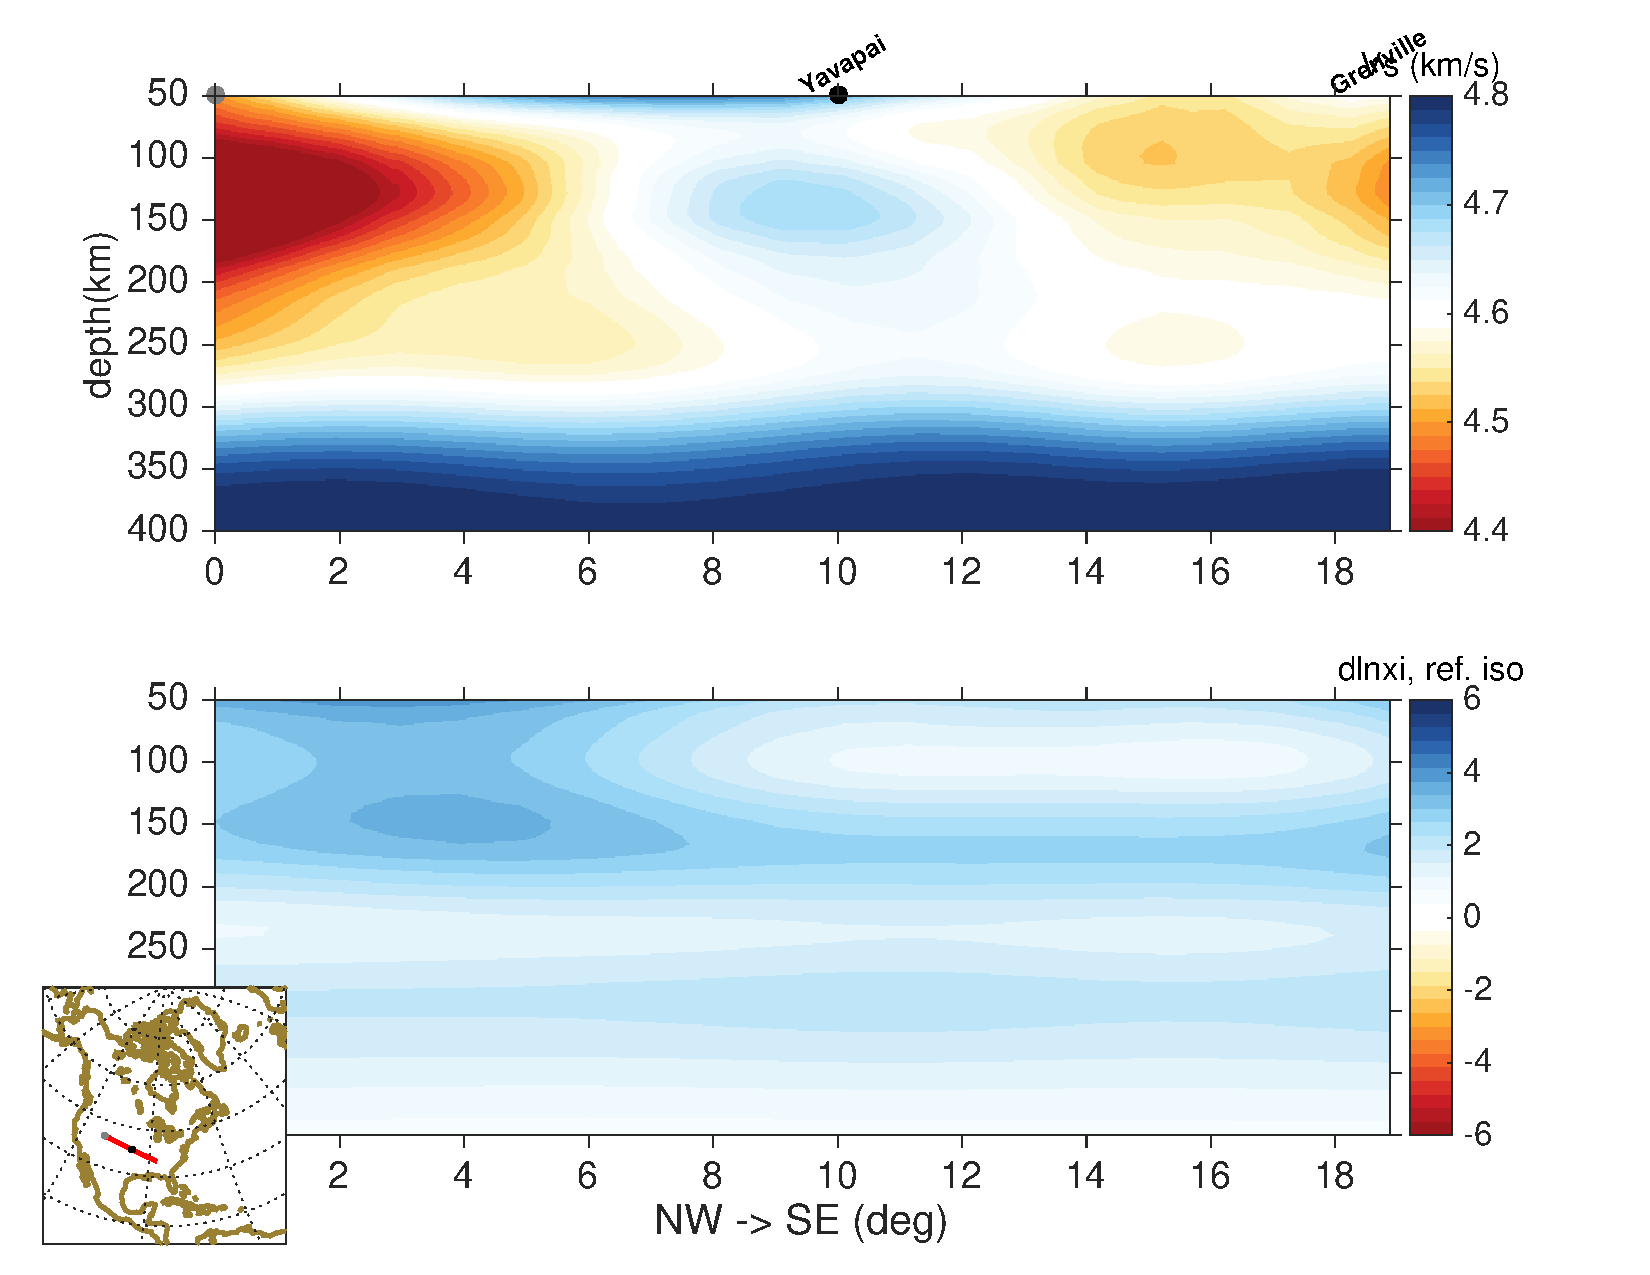
\includegraphics[width=\linewidth]{figures/profiles_NASEM3_vs_dxi_yava-maza_A.pdf}}
	% 	\end{minipage}
	% 	\hfill
	% 	\begin{minipage}{0.5\linewidth}
	% 		\centerline{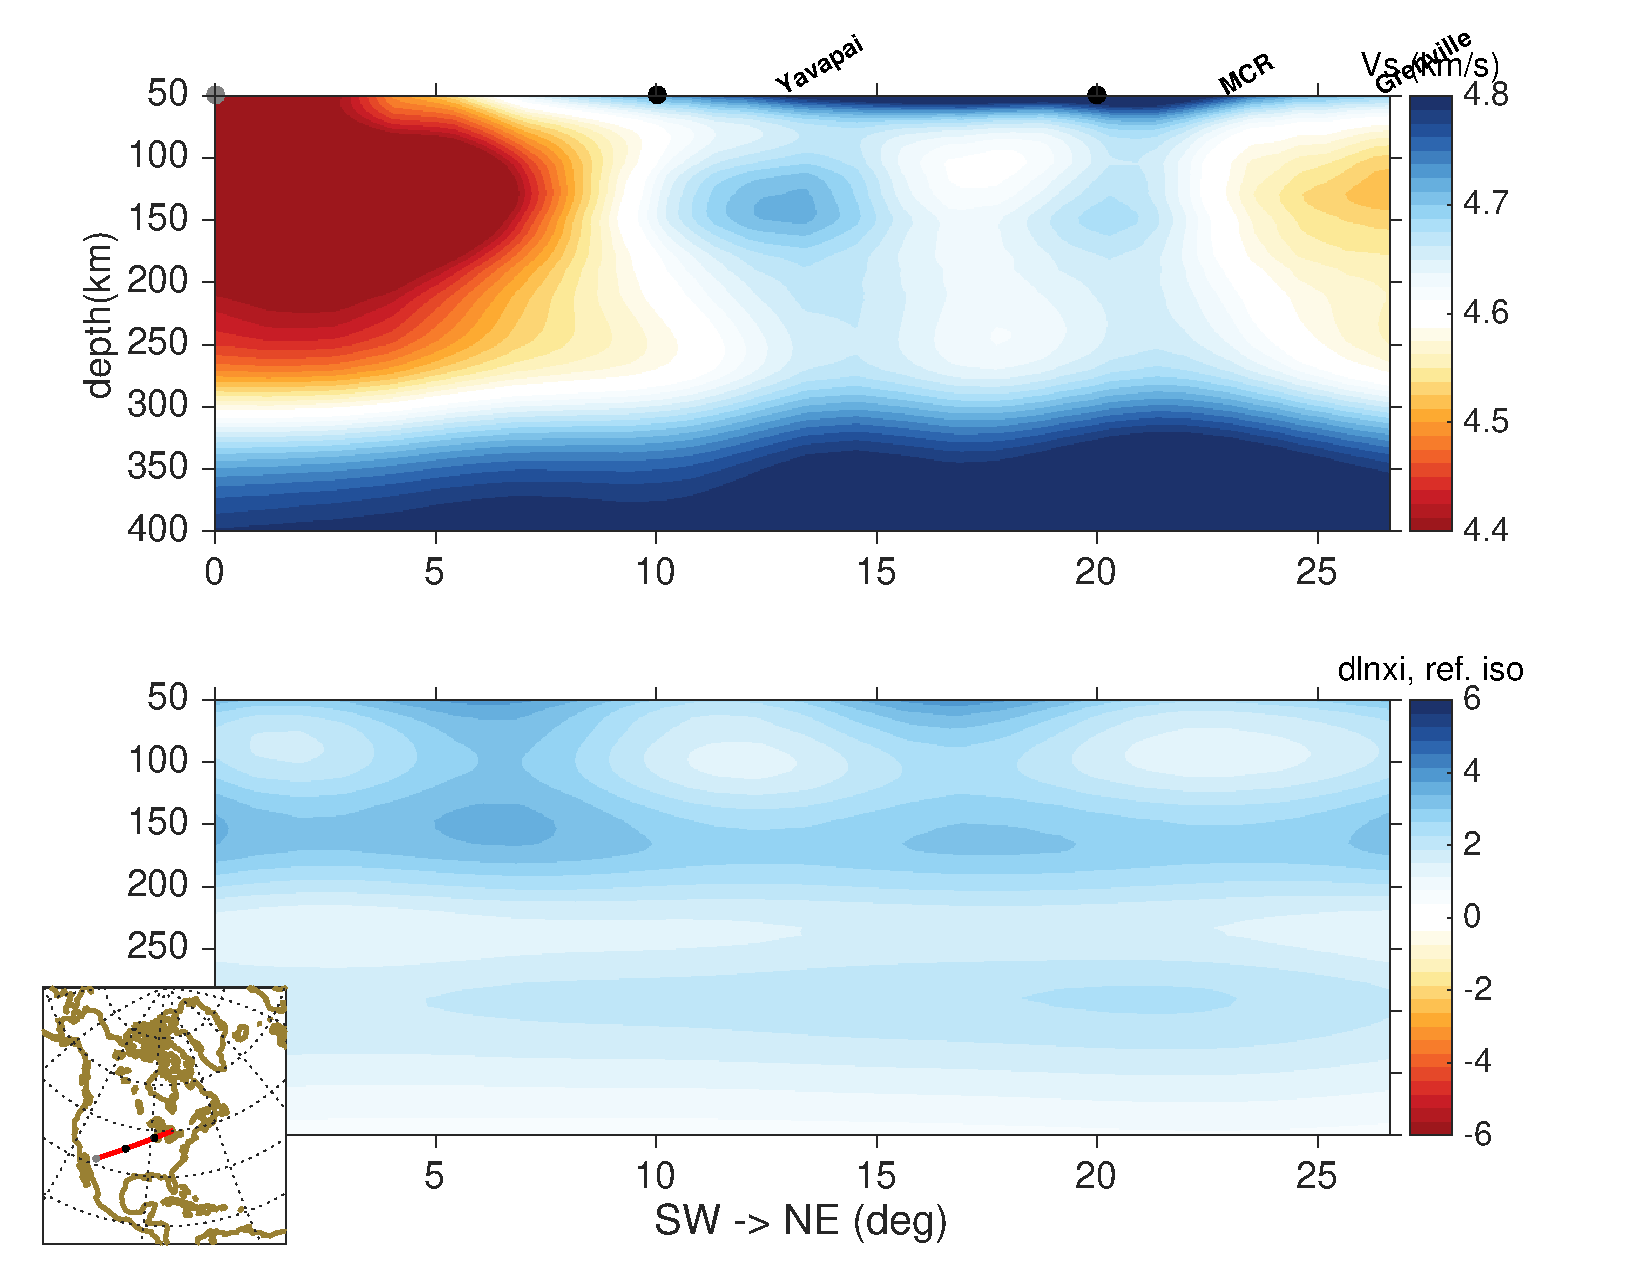
\includegraphics[width=\linewidth]{figures/profiles_NASEM3_vs_dxi_yava-maza_B.pdf}}
	% 	\end{minipage}

	% 	\caption{Cross Section of the Yavapai and Mazatzal lithosphere}
	% 	\label{yavacross}

	% \end{figure}


	Yavapai/Mazatzal/Granit-Rhyolite orogens from 1.8 to 1.6 Ga represent zones of accretion for Proterozoic material and mark the amalgamation of the archean cores. \citep{hoffman1988united} \\
	West to the RMF, the region shows low velocities influenced by the active tectonic with a radially positive gradient. 
	The north eastern part shows velocity anomalies slightly lower than the Archaean nucleus. Velocity maxima of $4.8km.s^{-1}$ are located shalower than $100km$. 
	Below, the radially negative gradient is observed and shows the same characteristic than the eastern Superior craton. It is interesting to note that, beneath Nebraska and Kansas, a high velocity anomaly of about $4.7km.s^{-1}$ is present until ca. $170km$ (while it is $120km$ in most of the region) where cretaceous aged kimberlites are sampled. 
	These kimberlites indicate a lithosphere thickness of about $160km$ and have been affected by asthenospheric upwelling related to the Mid-Continent Rift System. \citep{griffin2004lithosphere}



% Basal drag from Kaban 2015 cannot be visible from temperature sensitive shear waves model, we dont see it but it is normal.


\subsection{Surrounding oceanic} This section needs to be redone...

	Our inversion is focusing on the continental part, as shown in our spatial parameterization (i.e. see figure~\ref{density_coverage}) where the region is sampled by data.
	Ecxept the oceanic borders of NA, further away, the structure has not been updated from SEMucb\_wm1 \citep{french2014whole}. 

	\subsubsection{Eastern Passive margin}
		As in \cite{schaeffer2014imaging,yuan2014lithospheric,james2014rayleigh,silveira2002anisotropic,mocquet1990three}, we observe along the negative anomaly structure following the Appalachian continental shelf, a stretched positive anomaly structure from the Suwanne terrane in Florida to the Avalonian terranes of New-Scotland. 
		At $60km$ it is made of several blocks of at most $+3\%$ anomalies emdedded in a $+2\%$ structure. At $150km$, the structure is split into 2 blocks by a slow anomaly comprising both the Great Meteor (GMT) and Bermuda tracks, and further southeast, the Low Velocities Fingers (LVF) observed in \cite{french2013waveform}. 

		Such structure would correspond to late proterozoic gondwanian continental terranes that formed during the Pan African orogenesis \citep{kennedy1964structural} and remained attached to the North American margin during the opening of the Atlantic ocean. \citep[e.g.][]{thomas2006tectonic}
		On the continental shelf, authors \citep[e.g.][]{o1983avalon,nance2002cordilleran} identified the west Avalonian terranes of pan-african affinity as in Florida \citep[see][]{smith1982review} that might have been underlayed by a thin (ca. $100km$) lithosphere before the Pangaea assembling. \citep{mckenzie2015lithospheric}

		Fast anomalies are observed beneath the whole gulf of Mexico down to $150km$ deep. Despite the proximity with pan-african lithosphere, such high velocity anomalies represent older than $ca. 150Ma$ oceanic lithosphere. \citep{muller2008age,pindell2009tectonic}
		-- No Magnetic anomalies recorded as in Pan African, Oceanic seafloor according to Pindel --


% \subsubsection{Bermuda low velocity channel} 
% A low velocity anomaly is observed within the Atlantic ocean plate beneath the bermuda hotspot at $60km$ deep. Deeper, the slow anomaly broadens and is elongated along the absolute plate motion from the atlantic ridge to the Mid-Continental rift. This feature, parrallel the Absolute Plate Motion (APM) corresponds to the Low Velocity Fingers (LVF) introduced by \cite{french2013waveform} and it shows highest negative anomalies between $100km$ and $200km$ and seems to vanish below $250km$. 

% While in \cite{french2013waveform}, the North Atlantic LVF was stopped at the shelf of the US, our model shows that the slow velocity anomaly goes further through the continental lithosphere with a contrast of $-2\%$ to $-3\%$ compared to the surrounding cratonic root. 

% En regardant mieux les cartes, je ne suis pas sur a 100\% Le LVF semble se diriger vers Bermuda. Il y a une faible anomalie qui fait le lien vers GMT mais latendance general de l'anomalie GMT Bermuda LVF ne semble pas etre la meme chose. Je prefere finir la partie GMT et comprendre les mecanismes, lire plus de biblio lies aux LVF et faire les liens. (Pour aller plus loin que Huaiyu2014 et Scaeffer2014)

\subsubsection{The Great Meteor track}
	\begin{figure}
		\centerline{\includegraphics[width=\linewidth]{figures/profiles_NASEM3_vs_dxi_GMTrack.pdf}}

		\caption{Cross Section of the lithosphere along the Great Meteor track based on \cite{heaman2000timing} construction}
		\label{gmtcross}

	\end{figure}

	Our model images a slow velocity anomaly in agreement with the reconstruction of the Great Meteor Track (thin red line in figure ~\ref{3d-VS}) proposed by \cite{heaman2000timing}.
	Below $100km$ the pan african lithosphere is cut in two by a slow velocity anomaly beneath the New England seamounts (youngest part of the GMT). Further East, the slow anomaly follows the GMT crossing the continental shelf, Appalachian and Grenville orogens down to $200km$. 
	This slow anomaly corresponds to the V-shape dent, or divot, observed by \cite{lee1997upper} who explained the feature by the presence of water in the mantle. 
	We observe at $250km$ that the slow anomaly go further inland and crosses the Superior Craton northward until the Hudson bay following the GMT.
	See the cross section along the re-built GMT in figure ~\ref{gmtcross}.

	\cite{heaman2000timing}, based on $U-Pb$ perovskite age determinations of kimberlites, proposed a progressive southeastward younging of kimberlite magmatism throughout much of eastern North America. Considering it as a strong support for small volume mantle melting that have occurred along the continental portion of the Mesozoic Great Meteor mantle plume hotspot track initiated during the opening of the North Atlantic Ocean at about $200Ma$. \citep[See figure 4. in][]{heaman2000timing}

	\cite{davies1994thermomechanical} described a process of thermo-mechanical erosion which involves heating-softening of the lithospheric base by a plume tail, followed by mechanical removal of the material due to convective transfer. \citep{rondenay2000lithospheric}
% This hypothesis is based on different points:
% \begin{itemize}
% \item The lithosphere is moving above a fixed mantle where plume originate \citep[e.g.][]{morgan1972deep}
% \item Age progression along seamounts \citep[see for example][]{crough1980kimberlites,morgan1983hotspot,duncan1984age,sleep1990monteregian}
% \item Concordance between kimberlite ages and the continental drifting rate of North America. \citep{crough1980kimberlites,duncan1984age}
% \item Evidence of hotspot related uplift along both continental and oceanic structures. \citep{crough1981mesozoic,sleep1990monteregian}
% \item Similarities in initial Sr and Nd isotopic ratios between land and sea portions. (Foland et al., 1988)
% \end{itemize}

% Continuity: 
% Chercher anomalie de flux thermique (Jaupart 2000 2002 2014) ne montrent rien
% Parler de l'hypothese rifting of the continental plate qui est en opposition avec Mantle plume.
% -- Lien avec Vs (effet thermique/chimique/fabrics) ou il faudrait prendre en compte les effets anharmonicity/anelasticity. Voir Ebinger et Sleep 1998
% -- Haydar voit une anomalie negative de Q dans la region Great Meteor + Finger!! 
% -- Trouver model de conductivite, anomalie de Gravi? Pour appuyer 
% -- Faire le lien avec Kaban 2015 Byriol 2016 Poritt 2014
% -- Fingers From SEMum2 se dirigent plus vers le Bermuda hotspot que GMT, Meme si il y a un lien entre les 2 a 150km.
% -- Aucune update du Model de GMT depuis Haeman 2000...
% This feature, parrallel the Absolute Plate Motion (APM) corresponds to the Low Velocity Fingers (LVF) introduced by \cite{french2013waveform} and it shows highest negative anomalies between $100km$ and $200km$ and seems to vanish below $250km$. While in \cite{french2013waveform}, the North Atlantic LVF was stopped at the shelf of the US, our model shows that the slow velocity anomaly goes further through the continental lithosphere with a contrast of $-2\%$ to $-3\%$ compared to the surrounding cratonic root. This slow anomaly corresponds to the V-shape dent, or divot, observed by \cite{lee1997upper}. 


% Some authors [Sykes,1978; Croughet al., 1980] have suggested a genetic relation between
% kimberlites and hotspot tracks, here defined as lin-
% ear, anorogenicvolcanic chains mapped over oceanic
% and young continental lithospheres. The termination
% of these features over thickening continental roots has been cited as evidence supporting the origin of hotspot tracks in the interaction of fixed mantle plumes with an overriding plate [Morgan,1972;Burke and Wilson,
% 1976; Crough et al., 1980; Sleep, 1990a; Duncan and
% Richards, 1991], although compelling arguments may also be made for association of hotspot tracks with an-
% cient rifts and subvertical lithospheric discontinuities [Curtie,1976;Sykes,1978;Anderson1,998

% Hotspot tracks preserve records of past plate motion and provide markers with which the relative motion between a plate’s surface and underlying mantle regions may be examined




% Quand tu vas parler de l'implication thermale et chimqieu il faut citer le boulot de Haydar avec son anomalue negative de Q. 


% At least two Mesozoic hotspot tracks have been postulated for eastern North America; the Juras- sic Verde and Cretaceous Great Meteor tracks [38^40,42,43]. According to Morgan [39], these two parallel and closely spaced hotspot tracks passed through Ontario and the New England region at slightly di¡erent times (c. 40 Myr apart). The location of the continental portion of these tracks is based on several lines of evidence includ- ing: (1) the current position of Atlantic Ocean hotspots; (2) the record of ocean £oor magnetic anomalies; (3) the assumption that the position of hotspots remains relatively ¢xed on Earth with time; and (4) the relative motions of North Amer- ica, South America, and Africa during the various stages recorded in opening of the Atlantic Ocean since about 200 Myr [50]. In the case of these Atlantic hotspots, the initial portion of the track typically begins on the continent and eventually moves toward the current oceanic position of the corresponding mantle plume.    


% \subsubsection{Gulf of Mexico}
% Fast anomalies are observed beneath the whole gulf of Mexico down to $150km$ deep. Despite the proximity with pan-african lithosphere, such high velocity anomalies represent older than $150Ma$ oceanic lithosphere.

 % \subsection{Previous models}
 % Since \cite{grand1984upper}, one well established feature within NA lithosphere is the contrast between the high velocity craton and the low velocity western active part. This feature is observed in many global models (e.g., \cite{megnin2000three}, \cite{shapiro2002monte},  \cite{panning2006three}, \cite{houser2008shear}  \cite{nettles2008radially}, \cite{kustowski2008anisotropic}, \cite{ritsema2010s40rts}, \cite{simmons2010gypsum}, \cite{lekic2011inferring}, \cite{debayle2012global}, \cite{schaeffer2013global}, \cite{french2014whole}) where the cratonic lithosphere is caracterized by higher than average (ca. $4.8 km.s^{-1}$) velocities down to at least $200km$ deep. 

 % Measurements of heat flux and heat production over North America ( e.g \cite{jaupart2014building} ) showed low heat flux (i.e $30-50 mW.m^{-2}$) compared to surrounding area, with a contribution at the base of the archean lithosphere brought by convection and a small internal contribution from heat producing elements (e.g \cite{michaut2007transient}). This indicates that the cratonic lithosphere that have cooled down by conduction through time can reach a $400km$ thickness and is cold (\cite{rudnick1998thermal} \cite{s2005archean}).


% Preservation of the keel through time:
% - depth 400-500km incompatible with sismo and thermobarometric models.
% - Diamond inclusions in kimberlites and Re–Os isotope analyses of peridotite xenoliths indicate that xenoliths with Late-Archean ages erupted from depths up to 200km.
% 	-  If we assume that these xenoliths represent samples of the cratonic keel, this suggests that cratonic keels formed soon after (or along with) the craton and that subcratonic lithosphere was cold as early as the Late-Archean
% 		- Thus, cratonic keels would have appeared to have formed soon after the craton formed and have moved with the craton, relatively undeformed, through time. 
% 		- However, recent evidence suggests that Re–Os ages may over-estimate the age of xenoliths because zircon grown, and presumably diamond, does not reset the Re–Os system. It is difficult, at best, to preserve the diamond stability conditions for 3 Gyr, even in a stable continental keel. Perhaps the apparent ages are over-estimates; this would eliminate the need to maintain stable, low temperature keels for time periods up to 3 Gyr in the dynamical modeling.

% Jordan's tectosphere
% root of the cratonic lithosphere have remained unmixed with the rest of the upper mantle.
% 	Problem: No positive geoid anomaly observed so no mass excess
% Roots composition must be different in term of composition and iron depleted
% Chemistry of the tectosphere is mechanically strong and buoyant as the submantle but chemically distinct
% The effect of composition offsets the increase in density that results from cooling, leading to the isopycnic hypothesis, cratons and keels are neutrally buoyant.
% 	Problem: Neutral buyancy is not sufficiant to stabilyse cratonic keels from the shearing of mantle flow.
% 			Thermal conduction is a slow process (for the cooling), it is unlikely that compositional process can balance thermal cooling through time that would lead to neutral buoyancy.
% 			Geodynamical models cant maintain a stable cratonic root through time.

% geochemistry measures
% 	Cold and dehydrated keels appear to be residual from varying degrees of partial melting over a range of pressure {}with some post depletion metasomatic activity (King 2005).
	
% 	Thermobarometric studies indicate that until ca. $175km$ the mantle is chemically depleted. \cite{kopylova1999petrology} 

% 	Beneath 175km peridotite more fertile: Top of the convective mantle or archean oceanic crust undeplating craton or metasomatic activities... Re-Os datattion on eclogites showed that they are older than some peridotites -> keels are subducted archean ocean crust. \cite{shirey2001archean}

% 	A number of petrological studies confirm the relative buoyancy of xenoliths thought to represent the composition of the keel [4,24,51–53]. Reconciling the petrological models of root composition with the seismic velocities remains elusive (e.g., [20,24]). Dehydration can lead to several order of magnitude increase in viscosity, relative to mantle at the same pressure and temperature conditions [54,55]. Hence if the cratonic keels represent the depleted residual from a large melting event, this would be consistent with the buoyant and viscous properties that are needed to maintain stable keels over a long time period.

% Electrical conductovity:
% The bootom of upper mantle is wetter than above beneath craton and dryer than ocean until 250km \cite{yang2015three} \cite{hirth2000comparison}
% Jordan [23] hypothesized that subcratonic keels or
% roots are attached to the cratonic lithosphere and that
% these roots or keels have remained isolated from and
% unmixed with the rest of the mantle since the
% formation of the craton. If the cratonic root is a thick
% thermal boundary layer and the subcratonic mantle is
% average upper mantle composition, there should be a
% 10-m positive geoid anomaly over cratons [29].
% Because there is no correlation between continents
% and the geoid [30–32], the subcratonic mantle must be
% compositionally distinct from the surrounding upper
% mantle. Jordan called this subcratonic material tectosphere
% to distinguish it from normal upper mantle. In
% the tectosphere hypothesis these keels are chemically
% distinct from the convective mantle and are both
% compositionally buoyant and mechanically strong.
% The effect of composition offsets the increase in
% density that results from cooling, leading to the
% disopycnicT hypothesis [33]—cratons and keels are
% neutrally buoyant. Numerical studies have clearly
% demonstrated that neutral buoyancy is not sufficient to
% stabilize cratonic keels from the shearing of mantle
% flow. Thermal conduction is a slow and continuous
% process and it seems highly improbable that a
% compositional process would exactly balance thermal
% cooling through time, leading to neutral buoyancy at
% all depths envisioned in the isopycnic hypothesis.
% While both strength and buoyancy act to stabilize
% keels in theory, it has been quite challenging to
% produce geodynamical models that maintain stable
% cratonic keels in a convecting mantle over several
% billion years of mantle evolution (e.g., [3] and see
% later section on craton stability).

% In the steady state thermal conditions that prevail in old continents, the man- tle heat flux, i.e., the heat flux at the Moho, is the sum of the heat flux at the base of the lithosphere, which is brought by mantle convection, and heat generated by heat producing elements in the lithospheric mantle. The first contribution originates deeper than 200 km and potential lateral variations would get smoothed out by horizontal diffusion. The contribution of heat producing elements in the lithospheric mantle is very small, as shown by xenolith studies [Michaut et al., 2007], and horizontal anomalies would also be smeared out. Joint analysis of surface heat flux data and seismic wave velocity variations confirms that Moho heat flux variations are constrained to be less than about ± 3 mW m−2 , so that the total variation is 6 mW m−2 across the province [Perry et al., 2006b; Lévy and Jaupart, 2011].

 % \subsection{Craton caracteristic}


 % Through times, Lauretia craton remained undeformed while being part of the earliest supercontinent Nuna-Columbia \citep{meert2012whats}, then Rodinia and finally Pangaea.  

% Archean part more buoyant than proterozoic one
% The archean province may reflect a relatively depleted underlying mantle lithosphere.
% The presume secular decline in mean temperature of the asthenosphere impliesa greater depth and volume of melting accompanying mantle upwelling in the Archean, and consequently thicker, more depleted mantle lithosphere.

% Most importantly, the 2.7 Ga age of the Greenland eclogites supports the observation by Shirey and Richardson (2011) that mantle eclogite materials older than 3.0 Ga appear absent from the cratonic record. They suggest that the appearance of cratonic eclogites in most cratons after 3.0 Ga marks the onset of the Wilson Cycle of plate tectonics, when more frequent subduction and collision events became the most prominent continental growth mechanism. (Tappe et al., 2011)

% Previous studies
% Link with upper mantle tomography
% layering and radial intro to aximuthal


% In the early 1960s, theoretical work (e.g. Anderson 1961) on the dispersive properties of transversely isotropic media suggested that radial anisotropy in the upper mantle could have a pronounced ef- fect on the shape of surface wave dispersion curves and could lead to an apparent discrepancy between Love and Rayleigh wave data.

% For  more  than  thirty  years,  seismologists  have  imaged  the  earth's  interior  using  seismic
% waves generated by earthquakes,  and traveling through di erent structures of the planet.
% A  remaining  challenge  in  seismology  is  to  interpret  the  recovered  Earth  models  in  terms
% of physical properties (e.g.  temperature, density, mineral composition) that are needed for
% understanding  mantle  dynamics  and  plate-tectonics.   For  example,  a  region  of  slow  wave
% speed can be either interpreted as anomalously warm, or rich in water, or iron.
% Although seismic waves are sensitive to a large number of visco-elastic parameters as well
% as density, the mantle models constructed from seismic tomography are only parameterized
% with a few physical parameters, for example average isotropic shear wave velocity and radial
% anisotropy (e.g. French et al., 2013). This is because given the available information observed
% at the surface, there is not enough resolution to entirely describe the local elastic tensor.  In
% addition to the limitednumber of resolvable elastic (and anelastic) parameters, there is also
% the question of spatial resolution, namely the smallest spatial scale at which heterogeneities
% can be imaged.
% The  number  of  independent  elastic  parameters  that  can  



% \section{Methodology}
% % \subsection{Kernels}
% In the continuity of previous work (e.g Marone et al.,2007; Yuan et al.,2011; Yuan et al., 2014) we invert 3-component fundamental and overtone surface waves in the time domain to image North American upper mantle 3D structure using an hybrid inversion scheme. \\
% Inferring the elastic structure of the earth from the analysis of propagating waveforms is a well-studied inverse problem in geophysics. 
% % A non linear inverse problem that can be solved iteratively, where the accuracy of the different solution's terms may come along with the expensiveness of their calculation. 
% Our inverse problem is solved iteratively following the generalized least-squares formalism of Tarantola and Valette, 1982. We define a discrete L2 misfit functional:

% \begin{equation}
% 2\Phi(m_{k}) = [d - g(m_{k})]^{T} C^{-1}_{d} [d-g(m_{k})] + [m_{p}-m_{k}]^{T} C_{m}^{-1} [m_{p}-m_{k}]
% \end{equation}

% where \ensuremath{m_{k}} represents the \ensuremath{k^{th}} iterative model estimate, \ensuremath{d} and \ensuremath{g(m_{k})} are the observed data and data predictions (time-discretized waveforms and period-discretized group velocities), \ensuremath{m_{p}} is the model prior (1D earth or 3D starting model), and \ensuremath{C_{m}} and \ensuremath{C_{d}} represent a priori model and data covariance operators respectively. 

% We solve for successive updates to the current model estimate \ensuremath{m_{k} \to m_{k+1}} following the update equation that minimizes $\Phi$, namely:
% \begin{equation}
% m_{k+1} = m_{k} + (C_{m}G^{T}_{k}C^{-1}_{d}G_{k} + I)^{-1} (C_{m}G_{k}^{T}C^{-1}[d-g(m_{k})]+ m_{p}-m_{k})
% \end{equation}
% We employ a hybrid waveform inversion scheme, in which “exact” forward modeling of the wavefield (i.e. the waveform elements of $g(m_{k})$ is achieved using the spectral element method (SEM: e.g. Komatitsch and Vilotte, 1998; Komatitsch and Tromp, 2002a,b), while approximate sensitivity kernels (i.e. elements of G) are calculated using non-linear asymptotic coupling theory (NACT: Li and Romanowicz, 1995). 

% NACT is a normal-mode perturbation approach, which takes into account coupling between modes both along and across dispersion branches, allowing the computation of 2-D broad-band sensitivity kernels which more rigorously reproduce the sensitivity of body waveforms to structure along the ray geometrical path in the vertical plane containing the source and the receiver.
% However, when the distance between a source and a station is below $15^{o}$, NACT breaks down and we instead use the more standard Path Average Approximation (PAVA). Developed by Woodhouse \& Dziewonski, 1984; PAVA kernels are sensitive to the average structure between the source and the receiver and along the great circle path, that is, the corresponding sensitivity kernels are ‘1-D’ in the vertical plane containing the source and the receiver. This approximation is best for single-mode seismograms, such as fundamental mode surface waves (Romanowicz, 2008).


% PAVA/NACT do not consider off great circle path sensitivity in the horizontal direction, which gives rise 
% to focusing and defocusing effects (e.g. Zhou et al. 2005). These effects are important for amplitude 
% fitting. Here, we are, however, primarily concerned with fitting the phase and for that, the 2-D effects in
% the vertical plane are dominant, especially for overtones. The dominance of 2-D effects in the
% vertical plane can be assessed by considering an asymptotic expansion of normal mode first order
% perturbation theory, which shows that 2-D coupling effects in the vertical plane are of zeroth 
% order, while focusing effects are of higher order (e.g. Romanowicz, 1987; Li \& Romanowicz, 1995; Romanowicz, 2008).

% On the other hand, we use the spectral element method to accurately compute the forward seismic wavefield $g(m_{k})$. 
% Lekić \& Romanowicz., 2011 showed, that using approximate methods, such as normal mode perturbations theory, to calculate synthetic seismograms can introduce significant errors in the modeling of the wavefield in a heterogeneous 3-D earth. These errors can be seen as additional noise in the inversion and may introduce some model dependent errors. In that situation, convergence of the inverse problem can be compromised. We use a modified version of the spectral element code RegSEM (Cupillard et al., 2012) which initially was designed to calculate synthetic seismograms in a $90^{o} \times 90^{o}$ area within which both receivers and event sources are located. RegSEM takes into account effects of the oceans, topography / bathymetry, ellipticity, gravity, rotation and anelasticity. It also includes Perfectly Matched Layers (PML) absorbing boundary conditions, which allow us to restrict the computation laterally and radially to the region of interest with the vanishing of spurious reflections at the borders. (Patera \& Vilotte, 2005)

% Using only regional events is an opportunity to image the North American upper mantle without the influence on the wavefield of the global 3-D structure. However the current data coverage from a pure regional data set is not sufficient to constrain our region. To address this problem, we chose to include teleseismic events and developed a new method in order to calculate teleseismic synthetics where, through iterations, the wavefield is calculated only in the region of interest by the use of secondary sources.
% Developed by Masson et al., 2013, the idea is to construct an equivalent of time-reversal mirrors (Fink et al., 1989) at the boundary of our region of interest where the wavefield is then re-generated forwardly. 
% Time reversal is a two step process. First, waves propagating in a medium from a source are recorded thanks to an array of transducers (also named time-reversal mirrors). Second, after having reversed in time our records, transducers emit back into the medium toward the source where the ernergy is refocused in time and space. The feasability of such procedure relies in the reciprocity in space and reversibility in time of the wave equation. (Robertson \& Chapman, 2000) 

% % As in Robertson \& Chapman, 2000 we use a two step method. The first step performs wave propagations in the global medium, then as a second step the wavefield is used as an input (time-reversal mirrors) to obtain the wavefield into the medium under study. 

% In the elastic case, the ideal response of a time-reversal mirror can be expressed in the frequency domain with the use of the Helmotz-Kirchhoff representation theorem:
% \begin{equation}\label{eq:repres}
% \begin{split}
% 	u_{i}^{*}(\bm x) =&  \int_{V} G_{in}(\bm x, \bm x')f_{n}^{*}(\bm x')dV' \\
% 	 +& \oint_{S} G_{in}(\bm x, \bm x') n_{j} C_{njkl} \partial_{k}^{'} u_{l}^{*}(\bm x') dS' \\
% 	 -& \oint_{S} u_{n}^{*}(\bm x') n_{j} C_{njkl} \partial_{k}^{'} G_{il}(\bm x, \bm x')dS'
% \end{split}
% \end{equation}

% where $u$ is the displacement vector, $G_{in}(\bm x, \bm x')$ is the Green's tensor denoting the displacement at location $\bm x$ in the $i$ direction due to a unit point source at $\bm x'$ in the $n$ direction, $C_{ijkl}(\bm x)$ is the stiffness tensor at the $\bm x$ location, $\partial_{k}^{'}$ stands the derivative with respect to the $x_{k}^{'}$ coordinate and the star symbol (*) stands for the complex conjugate. Eq.\ref{eq:repres} shows that, if the exciting force $f_{n}(\bm x')$ is known throughout the volume $V$ and that the wavefield $u_{i}(\bm x)$, the associated traction $n_{j} C_{njkl} \partial_{k}^{'} u_{l}(\bm x')$ are known on the surface $S$; we are then able to regenerate the wavefield anywhere within the volume $V$. (Masson et al., 2013)

% Masson et al., 2013 proposed to introduce a spatial window function into the wave equation (original wavefield) in order to determine the exciting forces, that applied to the surface $S$, will generate the response $u_{i}(\bm x)$ defined in equation \ref{eq:repres}. 

% Starting with the wave equation in the frequency domain:

% \begin{equation}\label{eq:wavefreq}
% 	\rho \omega^{2} \bm u_n + \partial_j (C_{njkl}\partial_k \bm u_l) = -f_n,
% \end{equation}

% the generated wavefield in $M \in V$, is defined as:

% \begin{equation}\label{eq:um}
% 	\bm u^M (\bm x ,t) = \bm u(\bm x ,t)\omega(\bm x).
% \end{equation}

% with the use of a bi-valued function $\omega$:

% \begin{equation}\label{eq:window}
% 	 \omega(\bm x) = \left\{\begin{array}{ll}
% 						1 	&\mbox{ for all \quad $\bm x \in M$} \\
% 						0   &\mbox{ for all \quad $\bm x \notin M$}
% 						\end{array}
% 						\right.
% \end{equation}

% such as:


% \begin{equation}\label{eq:um_in_u}
%  \bm u^M (\bm x ,t) = \left\{\begin{array}{cl}
% 						\bm u (\bm x ,t) &\mbox{ for all \quad $\bm x \in M$} \\
% 						0                &\mbox{ for all \quad $\bm x \notin M$}
% 						\end{array}
% 						\right.
% \end{equation}

% where $M$ is the regional subvolume bounded by $\delta M$ within the global volume $V$.

% The mirror's excitation force that generates $\bm u^M$ is introduced as:
% \begin{equation}\label{eq:exc_force_reg}
%  	f_n^M = -\rho \omega^2 \bm u_n^M - \partial_j (C_{njkl}\partial_k\bm u_l^M)
%  \end{equation} 

%  Using eq. \ref{eq:wavefreq} - \ref{eq:exc_force_reg} and after developing:
%  \begin{equation}
%    	f_n^M = \omega f_n - C_{njkl} \partial_{j}\omega \partial_k u_l - \partial_j(u_l C_{njkl} \partial_k \omega).
%  \end{equation}

%  Finally, convolving eq. \ref{eq:exc_force_reg} with the Green's function of the medium and then integrate over the volume (see Masson et al., 2013 for a detailed derivation) gives :

%  \begin{equation}\label{eq:umfinal}
%  \begin{split}
%   	u_{i}^{M}(\bm x) =& \int_{M} G_{in}(\bm x , \bm x{'})f_{n} (\bm x') dV' \\
%   					 +& \oint_{\delta M} G_{in} (\bm x, \bm x') n_{j} C_{njkl} \partial_{k}^{'} u_l(\bm x')dS' \\
%   					 -& \oint_{\delta M} u_{n}  (\bm x') n_{j}   C_{njkl} \partial_{k}^{'} G_{il}(\bm x, \bm x')dS'
%  \end{split}
%  \end{equation} 

% In practice, one global simulation per event is needed to generate such mirrors, they are then used as secondary sources to generate the wavefield in our region of interest. These secondary sources are calculated once and for all. The main advantage of using such a method lies in the fact that we update the elastic structure of the region iteratively, we only need to calculate synthetics in the region. Since we're not updating the global structure (following the zeroth iteration ) of the earth but only North America, this allow us to save significant computation time and therefore attain shorter periods.

% The hybrid inversion scheme represents a compromise between speed and accuracy. The use of exact numerical methods to calculate the wavefield remains expensive, while waveform partial derivatives computed using NACT are approximate and inexpensive. Despite the approximate nature of NACT, we point out two important properties: sensitivity kernels, that are recalculated at each iteration in the current 3-D model) accommodate non-linearity due to multiple forward scattering (Romanowicz et al., 2008); and it includes finite-frequency effects in the 2D great-circle plane, critical to modeling surface-wave overtones and long-period body waves (Li and Romanowicz, 1995). 

% % \subsection{Effect of the crust}
% % From Scott's thesis 
% % Because SEM simulations are so precise, we require a model of crustal structure that accurately predicts the seismic response of the earth’s crust – particularly for highly sensitive fundamental- mode surface waves. Indeed, fidelity to crustal effects is especially critical for accurate retrieval of anisotropic mantle structure, as often noted when discussing the shortcomings of standard linear crustal corrections (Bozdag and Trampert, 2008; Lekic ́ et al., 2010; Ferreira et al., 2010). Here, we adopt the smooth crustal mod- eling technique proposed in Lekic ́ and Romanowicz (2011) and later refined by French et al. (2013). The thin layers of the earth’s crust slow down SEM computations considerably, particularly in the oceans. To mitigate this effect, we construct models of the crust that contain no interior discontinuities and are potentially thicker than the real crust in some regions. These smooth mod- els are calibrated to mimic the seismic response of the earth’s crust, as seen through observations of surface-wave group-velocity dispersion, by introducing crustal radial anisotropy (Backus, 1962; Capdeville and Marigo, 2007).
% % In the continents, our smooth crust matches the Moho depth of Crust2.0 (Bassin et al., 2000), with slight smoothing to avoid aliasing in the SEM mesh, while Moho depth saturates at 30 km in oceanic regions. A similar technique, but calibrated to mimic the dispersion of an a priori crustal model and not restricted to match continental Moho topography, has previously been shown to be effective for regional-scale waveform inversions (Fichtner et al., 2009). The disadvantages of such a technique are: (a) that the crustal model is only valid over the period range it is calibrated, in this case periods at or above 25 s, and (b) susceptibility to noise in the dispersion data upon which it is calibrated. The first concern should not be an issue for the 40 s and 60 s SEM modeling em- ployed here, confirmed in the global and North-American region validation simulations reported by French et al. (2013). To address the second concern, these authors produced ensembles of crustal models calibrated on dispersion data with realistic-amplitude syn- thetic noise added, and examined variation in the resulting SEM synthetics, concluding that such errors could not significantly af- fect long-period waveforms. Thus, we are confident that the crustal modeling approach is able to attain SEM speedup, while maintain- ing fidelity to the observed surface-wave dispersion characterizing crustal structure, and without negatively affecting the resulting long-period fundamental and higher mode waveforms and the re- sulting upper mantle shear velocity and radial anisotropy structure.


% \subsection{Parameterization}
% Propagation of seismic waves through an arbitrary Hookean medium depends on 21 parameters of the stiffness tensor,
% and inferring the values of all these parameters at all locations within the mantle is not feasible with available seismic data. 
% However, by approximating the Earth as a transversely isotropic medium with a vertical axis of symmetry ( VTI ), we can reduce the number of free parameters,
% while capturing the first order observation that horizontally polarized surface waves travel, on average, faster than vertically polarized ones (e.g. Anderson 1961; McEvilly 1964).  

% A VTI medium is described by density \ensuremath{\rho} and the five Love coefficients (\ensuremath{A}, \ensuremath{C}, \ensuremath{F},
%  \ensuremath{L} and \ensuremath{N} ) (Love 1927). 
% We parametrize our model in terms of \ensuremath{\rho}, the Voigt average isotropic shear ($V_S$) and compressional ($V_P$) velocities: \\
% \begin{align}
% V_{S} =& \sqrt{\frac{2V^{2}_{SV}+V^{2}_{SH}} {3}} \\
% V_{P} =& \sqrt{\frac{V^{2}_{PV} + 4V^{2}_{PH}}{5}}
% \end{align}

%  and the anisotropic parameters:

%  \begin{equation}
%  \xi = \frac{N}{L}, \quad \varphi = \frac{C}{A}, \quad \eta = \frac{F}{A-2L} 
%  \end{equation}
 
% Love and Rayleigh waves are primarily sensitive to shear wave structure, whereas their sensitivities are significantly weaker for other elastic parameters (Dahlen \& Tromp 1998). 
% Thus, we decrease the number of parameters of interest by choosing not to invert for lateral variations in the poorly constrained $V_{P}$ $\varphi$, $\rho$ and $\eta$ parameters. 
% Instead, we parametrize the elastic structure of the mantle in terms of $V_{S}$ and $\xi$.
% The parameter $\eta$ governs the variation of wave speed at directions intermediate to the horizontal and vertical. 
% When $\eta$ and $\varphi$ are approximately equal to one, which is very likely the case in the mantle, we can approximately relate Voigt average velocities to those of vertically and horizontally polarized waves.
% Following Montagner \& Anderson, 1989 we impose an a priori information on other parameters perturbations by scaling them with inverted parameters:

% \begin{equation}
% \frac{\delta(V_{P})}{\delta(V_{S})} = 0.5, \quad
% \frac{\delta(\rho)}{\delta(V_{S})} = 0.33, \quad
% \frac{\delta(\eta)}{\delta(\xi)} = -2.5,   \quad
% \frac{\delta(\varphi)}{\delta(\xi)} = -1.5,   \quad
% \end{equation}

% We opt for $V_{S}$ and $\xi$ parameterization instead of the more traditional $V_{SV}$ and $V_{SH}$, to avoid additional uncertainties on the amplitude and possibly even sign of the anisotropic parameter $\xi$ introduced by damping in the inversion process. (Marone \& Romanowicz, 2007)
% Indeed, if $\xi$ is computed after the inversion from the derived $V_{SV}$ and $V_{SH}$, its value can be biased by the different effect of damping on the two velocity parameters. ( Panning \& Romanowicz; 2006).

% In theory, the retrieved radial anisotropic model could be biased by the presence of azimuthal anisotropy, neglected at the present stage of this study. In practice, with sufficient azimuthal coverage, this possible effect is reduced because the azimuthal variations will be averaged out at each point of the model. This study, limited to radial anisotropy, should be regarded as a first step towards a more complex model of anisotropy, where the assumption of a vertical symmetry axis will be dropped and which will, therefore, still be characterized by radial anisotropy but with a symmetry axis with an arbitrary orientation (e.g. Montagner \& Nataf 1988).\\
		
% From the Core Mantle Boundary up to the Moho, the model is expressed on 26 cubic splines $\nu_{q}(r)$ defined in Megnin \& Romanowicz (2000), though we invert for structure only in the top 16 splines; deeper structure is fixed to that of our starting model $SEMucb_wm1$ (French \& Romanowicz, 2014). 
% The knot locations are at radii: 5690, 5810, 5910, 5990, 6061, 6101, 6131, 6161, 6191, 6221, 6241, 6261, 6281, 6301, 6321, 6341 km. 
% Laterally, we parametrize our model spatially in terms of spherical splines $\beta_{p}(\theta, \phi))$ (Wang \& Dahlen 1995). 
% Thus, the value of a given model parameter $m$ at any location in the Earth $(\theta, \phi, r)$ can then be calculated from a set of spline coefficients $m_{pq}$:

% \begin{equation}
% m(\theta,\varphi,r) = \sum_{p}\sum_{q}m_{pq}\beta_{p}(\theta,\varphi)\nu_{q}(r)
% \end{equation}

% The splines are a local basis, and thus help minimize the mapping of structure in one region into structure in distant regions, which can be an undesirable effect of global parametrization such as spherical harmonics (Lekic et al., 2011) .
% % In general when parameterizing our model, we put strict a priori constraints on the minimum length scale of structure allowed in our model. This truncation results in spectral leakage (aliasing) of short scale heterogeneity into longer length scales (Trampert \& Snieder 1996), though the use of splines reduces this aliasing when compared to spherical harmonics or spherical pixels (Chiao \& Kuo 2001). To further reduce the aliasing of retrieved structure, we allow structure to vary at shorter length-scales than those that we can reasonably expect to image and interpret (Spetzler \& Trampert 2003).

% In our regional tomographic studies, the mesh for the target region can be refined by adding knots halfway between two neighboring grid points, until the desired knot spacing has been reached, while maintaining a coarser mesh throughout the rest of the globe (Marone \& Romanowicz 2007a). This approach allows flexibility: the grid spacing can, for instance, be chosen as a function of the data coverage. Therefore, we maximize the resolution within the ideally sampled region, without need for over parameterizing the areas with insufficient data density. For the $V_{S}$ parameter we use a regional level 7 spherical grid (~1 degree knots spacing) and level 6 ( ~2 degree ) for $\xi$. 

% \subsection{A priori information}
% When solving an inverse problem, the importance of the a priori information depends greatly on the use one plans for the estimated model parameters.
% If one simply wants one example of a solution to the problem, the choice of a priori information is unimportant. However, if one wants to develop arguments that depend on the uniqueness of the estimates, the validity of the a priori assumptions is of paramount importance. (Menke, 2012)

% As a starting model, we opted for the global 3D radially anisotropic shear wave velocity model $SEMUCBwm1$ (French \& Romanowicz, 2014). This global whole mantle model was built in the continuity of SEMum generation models (Lekić \& Romanowicz, 2011) with an extended data set of :
% \begin{itemize}
% 	\item 3 components 60-400s periods waveforms
% 	\item 3 components 30-400s periods body-waves 
% 	\item group-velocity dispersion maps 25-150s 
% \end{itemize}


% Concerning the isotropic structure, the a priori information on which SEMum is based on is a VTI 1D earth model. The idea was to fit long-period ($T > 60 s$) waveforms (Cammarano \& Romanowicz 2007) starting from one of the physical reference models of Cammarano et al. (2005), which are calculated from a fixed composition (dry pyrolite) and a thermal profile using the elastic and anelastic properties of principal mantle minerals.

% As for the the anisotropic part, the a priori information of $\xi$ was obtained by testing several values against a set of observed frequencies of spheroidal and toroidal modes, keeping fixed the elastic structure. 
% In this process, $\xi$ was allowed to be stronger or equal to 1 (isotropic case) at depth shallower than 320 km as verified in numerous previous seismic studies (Dziewonski \& Anderson 1981).

% When solving the inverse problem, we also include a priori information on the model in a covariance matrix $C_{M}$. It specifies the expected deviation of true mantle structure from that specified by our starting model. This matrix is defined by the variance $\sigma^{2}_{0}$ (the diagonal entries) and the horizontal and vertical correlation lengths, $h_{0}$ and $v_{0}$, associated with each spline knot. 

%  These correlation lengths are spatially tuned according to data-coverage density and quality. As in \cite{lekic2011inferring}, the element of $C_{M}$ jointly describing the state of a priori information on model coefficients i and j is given by:

% \begin{equation}
% C_{m} = \sigma_{ij} exp(\frac{cos\Delta_{ij}-1}{h^{2}_{ij}}) exp(\frac{-2d^{2}_{ij}}{v^{2}_{ij}})
% \end{equation}

% where $\Delta_{ij}$ is the minor-arc distance separating model coefficients i and j, $d_{ij}$ their radial separation, and $v_{ij}$ and $h_{ij}$ the averages of their associated radial and lateral correlation lengths. 

% In order to increase image resolution, we allowed the horizontal length of correlations to vary between $100 km$ and $300 km$ for $V_{S}$; $300 km$ to $600 km$ for $\xi$. Thus, within the model, $h_{ij}$ can vary based upon an estimator for relative sensitivity. The idea is to take the diagonal of the approximated Gauss-Newton Hessian $G^{T}C^{-1}G$ associated with the data misfit term, to represent aggregate sensitivity of the data to each model coefficient. Contributions from different data type are weighted accordingly to the quality and uncertainty estimates appearing in the data covariance matrix $C_{D}$. These values are, in turn, used to select local correlation-length estimates by scaling to the interval between prescribed minimum and maximum values for a given model parameter. 

% \subsection{data}

% In this study, long-period waveforms and group velocity dispersion maps are used to constrain shear wave velocities and radial anisotropy in both crust and upper mantle of North America.

% The group-velocity dispersion data are from Ritzwoller et al., 2002 and are in the form of $1^o \times 1^o$ maps between 25 and 150s. The use of short period dispersion curves ( below 80s ) constrained our homogenized crustal structure, while the entire period range was included during the inversion of the mantle structure.

% The long-period waveform data set comprises Rayleigh and Love accelerograms including both fundamental and higher modes recorded on 3 components broad-band seismographs. 
% Fundamental modes are primarly sensitive to the first 300km while overtones have sensitivity into the transition zone. We used 2 different data sets: 

% \begin{itemize}
% 	\item a regional data set consisiting of 155 events $(4.5 < M_{w} < 6.0)$ where sources are located within the $90^o \times 90^o $RegSEM mesh.
% 	\item a teleseismic data set consisting of 122 events $(5.5 < M_{w} < 6.9)$ for which secondary sources are calculating around the $90^o \times 90^o $ RegSEM mesh using the procedure of \cite{masson2013numerical}.
% \end{itemize}
	
% Such data set, recorded at more than 2400 stations, provides an exellent azimuthal coverage of NA continent, with a total of 19.991 Love wavepackets, 55.176 Rayleigh wavepackets for fundamental modes, 82.809 overtones with 20 per cent from the T component and 63.179 wavepackets mixing fundamental and overtone energies.

% We filter accelerograms between 40 and 400s with corner frequencies at 53 and 250s, and separate them into wave-packets. Before inversio, the wavepackets are weighted according to their relative amplitudess, in order to avoid dominance by the larger amplitude fundamental modes in the inversion. In our weighting scheme, we also account for background noise, and path redundancy, as described in \cite{li1996global} This weighting step is crucial as it homogenizes the data coverage within the region and provides a way to construct the data covariance matrix $C_D$, which we approximate as a diagonal matrix.

\bibliographystyle{apalike}
\bibliography{/Users/Pierre/Documents/PHD/Thesis/biblio.bib}
%
\end{document}

%